\documentclass[a4paper, 12pt, twoside,openright]{book}
\usepackage[english, italian]{babel}
\selectlanguage{italian}
\usepackage[osf]{libertinus} %font generale del documento
\pagestyle{plain} %nessun heading o foot particolare
% Body size set by \documentclass (12pt); footnotes set to 10pt below = standard convention
\usepackage[a4paper,top=3cm,bottom=3cm,inner=3cm,outer=3cm]{geometry} %impaginazione e margini documento (symmetric: same margins on every page, no verso/recto shift)
\usepackage{graphicx, wrapfig} %gestione immagini e grafiche
\usepackage{array} % modificatori di tipo colonna (>{\raggedright\arraybackslash}p{...}) per le tabelle dell'appendice
\graphicspath{{images/}}
\usepackage{amsmath, amsfonts}  % Math and blackboard-bold (\mathbb)
\usepackage{booktabs}   % Per le linee orizzontali eleganti nelle tabelle (\toprule, \midrule)
\usepackage{longtable}  % Per le tabelle che si dividono su più pagine
\usepackage{pdflscape} % Per girare le pagine in orizzontale
\usepackage{float}           % For figure placement control
\usepackage[hidelinks,backref=page]{hyperref}  % \url{} plus "Cited on page(s)" back-links in the bibliography
\usepackage{microtype}  % Better justification and hyphenation, fewer overfull boxes
\emergencystretch=2em    % Allow extra interword stretch before an overfull line is emitted
\usepackage{xurl}       % Allows line breaking inside long URLs
\usepackage{glossaries}  % Hyperlinked glossary entries (\gls{}); page back-links to the text
\makenoidxglossaries
% Voci di glossario (definite nel preambolo per la modalità senza indice).
% La prima occorrenza di ogni termine nel corpo usa \gls{<label>}, che rende il
% termine e collega ipertestualmente al Glossario.
\newglossaryentry{dtu}{
  name={uso differenziale dei trascritti (DTU)},
  first={uso differenziale dei trascritti (DTU)},
  text={DTU},
  description={Si ha uso differenziale dei trascritti quando l'espressione relativa di più trascritti dello stesso gene cambia tra condizioni diverse \cite{young2024dtu}. È indipendente dai cambiamenti di espressione totale del gene, quindi non viene catturato dall'analisi dell'espressione differenziale a livello genico e richiede una risoluzione a livello di trascritto per essere rilevato.}
}

\newglossaryentry{deg}{
  name={espressione genica differenziale (DGE)},
  first={espressione genica differenziale (DGE)},
  text={DGE},
  description={L'analisi delle differenze nell'espressione totale di un gene---la somma dell'espressione di tutte le sue isoforme---tra gruppi di campioni. Misura l'output genico complessivo ed è cieca ai cambiamenti nell'uso relativo delle singole isoforme, che sono invece catturati dall'uso differenziale dei trascritti.}
}

\newglossaryentry{threePrimeEnd}{
  name={estremità 3'},
  description={L'estremità terminale di una molecola di RNA in cui termina la trascrizione; nell'mRNA è il punto in cui viene aggiunta la coda poli-A. Nei protocolli 3'-biased la chimica di cattura è ancorata a questa estremità, quindi i read coprono solo il frammento terminale di ciascuna molecola anziché l'intero trascritto.}
}

\newglossaryentry{threePrime}{
  name={sequenziamento 3'-biased},
  first={sequenziamento 3'-biased},
  text={3'-biased},
  plural={3'-biased},
  description={Una proprietà di alcuni protocolli di scRNA-seq (come 10x Genomics Chromium) in cui i read di sequenziamento derivano solo dal 3' terminale di ciascun trascritto. Poiché la qualità di lettura diminuisce con la distanza e la cattura è ancorata all'estremità 3' del trascritto, la copertura non si estende al corpo del trascritto, quindi le giunzioni di splicing interne non vengono mai osservate \cite{regan2022practical}.}
}

\newglossaryentry{isoformSwitch}{
  name={switch di isoforma},
  description={Un cambiamento, tra condizioni diverse, nell'uso relativo delle isoforme di un gene, per cui la frazione di espressione genica contribuita da una isoforma aumenta mentre quella di un'altra diminuisce. Riflette un'alterazione dello splicing alternativo o della trascrizione ed è quantificato dal cambiamento della frazione di espressione totale del gene attribuibile a ciascuna isoforma \cite{vitting2017isoformswitch}.}
}

\newglossaryentry{sparsity}{
  name={sparsità},
  description={La proporzione molto elevata di conteggi nulli nei dati di scRNA-seq.}
}

\newglossaryentry{dropout}{
  name={dropout tecnico},
  plural={dropout tecnici},
  description={Un conteggio nullo prodotto da un limite tecnico del saggio---cattura, retrotrascrizione o sequenziamento falliti---anziché dall'assenza reale del trascritto. È anche descritto come zero non biologico.}
}

\newglossaryentry{zeroInflated}{
  name={distribuzione zero-inflated},
  plural={distribuzioni zero-inflated},
  description={Un modello statistico per dati di conteggio che è una miscela di una massa puntuale in zero e di una distribuzione di conteggio standard (come Poisson o binomiale negativa). Si usa quando i dati contengono più zeri di quanti ne preveda la sola distribuzione di conteggio, trattando quegli zeri in eccesso come generati da un processo separato. Nello scRNA-seq il termine è stato applicato in modo incoerente, e il suo uso è dibattuto perché uno zero può riflettere un errore di misura o l'assenza reale di espressione \cite{sarkar2021separating}.}
}

% Nessun punto aggiuntivo tra una descrizione e il suo elenco di pagine.
\renewcommand*{\glspostdescription}{}

\newglossaryentry{countMatrix}{
  name={matrice di conteggi},
  plural={matrici di conteggi},
  description={Una tabella le cui righe indicizzano le feature (geni o trascritti) e le cui colonne indicizzano le cellule, in cui ogni voce registra quante molecole di quella feature sono state rilevate in quella cellula.}
}

\newglossaryentry{isoform}{
  name={isoforma},
  plural={isoforme},
  description={Una variante distinta di trascritto maturo prodotta dallo stesso gene tramite splicing alternativo.}
}

\newglossaryentry{scRnaSeq}{
  name={sequenziamento dell'RNA a singola cellula (scRNA-seq)},
  first={Sequenziamento dell'RNA a singola cellula (scRNA-seq)},
  text={scRNA-seq},
  description={Sequenziamento dell'RNA eseguito separatamente su migliaia di singole cellule, che rivela l'espressione di ogni cellula.}
}

\newglossaryentry{bulkRnaSeq}{
  name={bulk RNA-seq},
  description={Sequenziamento dell'RNA riunito da molte cellule in una sola volta, che media le differenze tra cellule.}
}

\newglossaryentry{fullLength}{
  name={sequenziamento full-length},
  description={Un approccio di sequenziamento che legge una molecola di RNA da un capo all'altro, anziché solo il frammento più vicino a una delle sue estremità.}
}

\newglossaryentry{read}{
  name={read},
  plural={read},
  description={Una breve sequenza nucleotidica prodotta dallo strumento di sequenziamento, che costituisce il dato grezzo dell'RNA-seq.}
}

\newglossaryentry{cellCluster}{
  name={cluster cellulare},
  plural={cluster cellulari},
  description={Un gruppo di cellule con profili di espressione simili, ottenuto raggruppando la matrice di conteggi. La maggior parte delle analisi a singola cellula confronta i cluster cellulari tra loro.}
}

\newglossaryentry{throughput}{
  name={throughput},
  description={Il numero di cellule che un singolo esperimento può processare in una corsa. È in compromesso diretto con la profondità di sequenziamento per cellula, perché uno strumento emette un numero fisso di read che deve essere diviso tra tutte le cellule catturate.}
}

\newglossaryentry{plateProtocols}{
  name={metodi su piastra},
  first={metodi su piastra},
  description={Un formato di scRNA-seq in cui ogni cellula è isolata nel proprio pozzetto di una piastra multiwell e i suoi trascritti sono catturati da un capo all'altro, così i read coprono l'intera molecola. Il formato preserva le giunzioni di splicing interne e raggiunge una profondità elevata per cellula, al costo di un throughput limitato a centinaia o poche migliaia di cellule.}
}

\newglossaryentry{dropletProtocols}{
  name={protocolli a goccia (dati a goccia)},
  first={protocolli a goccia},
  text={protocolli a goccia},
  description={Protocolli a singola cellula ad alto throughput che incapsulano ogni cellula insieme a una bead barcodata in una goccia di picolitri, così che decine di migliaia di cellule siano processate in una sola corsa. Sono il formato di scRNA-seq dominante e la loro chimica di cattura legge solo la coda di ciascun trascritto.}
}

\newglossaryentry{tagBias}{
  name={tag bias},
  first={tag bias},
  description={Un bias per cui ogni molecola viene letta da una sola delle sue estremità, così la copertura si concentra vicino a quell'estremità mentre l'interno del trascritto non viene mai osservato. Deriva da una chimica di cattura ancorata a una singola estremità, come nei protocolli a goccia con priming sulla coda.}
}

\newglossaryentry{cellBarcode}{
  name={cell barcode},
  plural={cell barcode},
  description={Una breve etichetta di DNA portata da ogni read di una data cellula, che ne identifica la cellula di origine. Consente di raggruppare i read di una corsa di sequenziamento riunita in profili di espressione per cellula.}
}

\newglossaryentry{umi}{
  name={Unique Molecular Identifier (UMI)},
  first={Unique Molecular Identifier (UMI)},
  text={UMI},
  plural={UMI},
  description={Una breve sequenza casuale legata a ciascuna molecola di RNA catturata prima dell'amplificazione PCR, così che le copie amplificate di una stessa molecola siano riconosciute e contate una sola volta.}
}

\newglossaryentry{pcr}{
  name={PCR},
  first={PCR (reazione a catena della polimerasi)},
  description={Reazione a catena della polimerasi: il passo di amplificazione che copia molte volte ogni frammento di cDNA catturato, così che le poche molecole recuperate da una cellula siano presenti in quantità sufficiente perché il sequenziatore le legga \cite{saiki1985enzymatic}. Poiché le copie superano in numero le molecole originali, il tag UMI è ciò che permette di ricondurle a un unico conteggio.}
}

\newglossaryentry{rna}{
  name={RNA (acido ribonucleico)},
  first={RNA (acido ribonucleico)},
  text={RNA},
  description={L'ampia classe di molecole di acidi nucleici trascritte dal DNA. Comprende l'RNA messaggero (mRNA), che porta le istruzioni per la codifica delle proteine, e gli RNA non codificanti, che svolgono ruoli strutturali o regolatori.}
}

\newglossaryentry{mrna}{
  name={RNA messaggero (mRNA)},
  first={RNA messaggero (mRNA)},
  text={mRNA},
  description={Il sottotipo di RNA che codifica proteine e che porta la sequenza di un gene al ribosoma.}
}

\newglossaryentry{rnaSeq}{
  name={sequenziamento dell'RNA (RNA-seq)},
  first={sequenziamento dell'RNA (RNA-seq)},
  text={RNA-seq},
  description={Una tecnica che determina la sequenza e l'abbondanza delle molecole di RNA in un campione; è la base dei protocolli a singola cellula discussi in questa tesi.}
}

\newglossaryentry{splicing}{
  name={splicing alternativo},
  first={splicing alternativo},
  text={splicing alternativo},
  description={Il processo con cui la lunga copia primaria di RNA di un gene viene accorciata e riorganizzata durante la maturazione. La copia contiene blocchi codificanti (esoni) e blocchi non codificanti (introni); lo splicing rimuove gli introni e unisce gli esoni fiancheggianti nelle giunzioni di splicing risultanti. Quando la selezione degli esoni varia tra i trascritti dello stesso gene, il risultato è più isoforme distinte.}
}

\newglossaryentry{mutualExclusivity}{
  name={esclusività reciproca},
  description={Due feature che compaiono raramente insieme nella stessa cellula (un'associazione negativa), in contrapposizione alla co-espressione.}
}

\newglossaryentry{gdi}{
  name={Global Differentiation Index (GDI)},
  first={Global Differentiation Index (GDI)},
  text={GDI},
  description={Una misura di specificità di cluster usata per identificare i geni marcatore e validare la qualità del clustering.}
}

\newglossaryentry{coexpression}{
  name={co-espressione},
  description={La tendenza di due feature (geni o trascritti) a essere rilevate insieme nelle cellule.}
}

\newglossaryentry{contingencyTable}{
  name={tabella di contingenza},
  description={Una tabella $2 \times 2$ che conta, su tutte le cellule, le quattro combinazioni di presenza e assenza di due feature; verifica se esse co-occorrono più o meno di quanto il caso preveda.}
}

\newglossaryentry{pseudoBulk}{
  name={aggregazione in pseudo-bulk},
  description={La pratica di sommare i conteggi di read su gruppi di singole cellule per simulare la profondità del bulk RNA-seq, recuperando potenza statistica a scapito dell'eterogeneità a singola cellula.}
}

\newglossaryentry{orthogonalValidation}{
  name={validazione ortogonale},
  description={Conferma indipendente di un risultato computazionale mediante una diversa tecnica sperimentale.}
}

\newglossaryentry{transcript}{
  name={trascritto},
  plural={trascritti},
  description={Una molecola di RNA copiata da un gene.}
}

\newglossaryentry{unsplicedTranscript}{
  name={trascritti non spliced/spliced},
  first={trascritto non spliced},
  text={trascritto non spliced},
  plural={trascritti non spliced},
  description={La prima copia di RNA di un gene, che contiene ancora i suoi blocchi non codificanti (introni); è anche detta trascritto primario o pre-mRNA. Il suo corrispettivo è il trascritto spliced, la stessa molecola una volta rimossi quei blocchi, ovvero la forma matura che viene tradotta in proteina.}
}

\newglossaryentry{spliceJunction}{
  name={giunzione di splicing},
  plural={giunzioni di splicing},
  description={Il confine creato quando due blocchi codificanti (esoni) vengono uniti dopo la rimozione del blocco non codificante interposto (introne). I read che attraversano una giunzione di splicing identificano quali blocchi sono stati uniti insieme.}
}

\newglossaryentry{gene}{
  name={gene},
  plural={geni},
  description={Un'unità funzionale del genoma che specifica una o più molecole di RNA.}
}

\newglossaryentry{protein}{
  name={proteina},
  plural={proteine},
  description={Una molecola costruita da una catena di amminoacidi che svolge il lavoro della cellula, tra cui catalizzare reazioni, trasmettere segnali e formare componenti strutturali.}
}

\newglossaryentry{genome}{
  name={genoma},
  description={L'insieme completo del materiale genetico di un organismo, scritto nel DNA e trasmesso di generazione in generazione. È organizzato in geni, le unità funzionali la cui espressione viene misurata.}
}
% Sopprime l'intestazione generata dal pacchetto; il capitolo fornisce la propria.
\renewcommand{\glossarysection}[2][]{}
% Indicazione di stampa: evidenzia i termini del glossario alla prima occorrenza.
\renewcommand{\glstextformat}[1]{\textit{#1}}

\usepackage{enumitem}   % Cleaner list spacing
\usepackage[nobottomtitles*]{titlesec}   % Heading spacing; keeps section titles off the page foot
\usepackage[hang,bottom]{footmisc} % Footnotes: hanging indent, no rule line, flush to page bottom
% Footnote styling: no rule line, smaller text, inset from main-text margin, hanging indentation
\renewcommand{\footnoterule}{}                        % no separator line between text and footnote
\renewcommand{\footnotesize}{\fontsize{10}{12}\selectfont}  % standard footnote size: 10pt for a ~12-13pt body
\begingroup\footnotesize\setlength{\footnotemargin}{2em}\endgroup  % footnotes inset from text margin (measured at footnote size)
\setlength{\footnotesep}{8.4pt}  % standard inter-footnote gap (bk12 default)
\setlist{topsep=0.6em, partopsep=0pt, itemsep=0.15em, parsep=0pt}  % Lists match paragraph rhythm
\titleformat{\section}{\Large\bfseries}{}{0pt}{}
\titlespacing*{\section}{0pt}{1.4em plus 1pt minus 1pt}{0.6em}
\titleformat{\subsection}{\large\bfseries}{}{0pt}{}
\titlespacing*{\subsection}{0pt}{1.1em plus 1pt minus 1pt}{0.4em}
\titleformat{\subsubsection}{\normalsize\bfseries}{}{0pt}{}
\titlespacing*{\subsubsection}{0pt}{0.9em plus 1pt minus 1pt}{0.3em}
% Avoid single orphan/widow lines at page boundaries; keep vertical flow unstretched
\widowpenalty=10000
\clubpenalty=10000
\displaywidowpenalty=10000
\raggedbottom
% Definition note placed at the bottom of the page where the concept first appears
\newcommand{\defn}[2]{\footnote{\textbf{#1:}~#2}}
\setlength{\parindent}{0pt}     % No paragraph indentation
\setlength{\parskip}{1em}       % Space between paragraphs
\setcounter{tocdepth}{1}        % Table of contents: chapters and sections only

\begin{document}
% Seed the core COTAN reference so it is numbered [1] under citation-order style
\nocite{galfre2021cotan}
% Front matter (roman page numbers)
\frontmatter
% Title page
\begin{titlepage} %crea l'enviroment
\begin{figure}[t] %inserisce le figure
    \centering
\includegraphics[width=0.98\textwidth]{marchio_unipi_pant541.png}
\end{figure}
\vspace{15mm} % Spazio leggermente ridotto

\begin{Large}
 \begin{center}
	\textbf{Dipartimento di Informatica\\ Corso di Laurea Triennale in Informatica\\}
	\vspace{15mm} % Spazio leggermente ridotto
    {\LARGE{TESI DI LAUREA TRIENNALE}}\\
	\vspace{10mm}
	{\huge{\bf Possiamo rilevare l'uso differenziale di trascritti (DTU) da scRNA-seq?}}\\
\end{center}
\end{Large}

\vfill % <--- QUESTO È IL TRUCCO. Distribuisce lo spazio in automatico senza far sbordare la pagina.

%minipage divide la pagina in due sezioni settabili
\begin{minipage}[t]{0.47\textwidth}
	{\large{\bf Relatori:\\ Prof.ssa Silvia Galfré\\ Prof. Corrado Priami}}
\end{minipage}
\hfill
\begin{minipage}[t]{0.47\textwidth}\raggedleft
	{\large{\bf Candidato: \\ Lorenzo Delitala}}
\end{minipage}

\vspace{15mm} % Spazio leggermente ridotto

\hrulefill

\vspace{5mm}

\centering{\large{\bf Anno Accademico 2025/2026 }}

\end{titlepage}
\chapter*{Ringraziamenti}
\addcontentsline{toc}{chapter}{Ringraziamenti}

Ai miei genitori, ai quali non lo dico abbastanza, ma il cui sostegno
incondizionato è qualcosa di cui sono immensamente grato.

\bigskip

A Niccolò, che influenza le mie scelte di vita da più di un decennio ormai.

\bigskip

A lui, insieme a Marchetto e a Bruno, va un grazie anche per aver reso questa
Triennale di Informatica decisamente più piacevole e divertente.

\bigskip

Ad Elena, per avermi supportato e sopportato
durante tutta la complessa fase di ricerca pratica, ed essermi stata accanto.

\bigskip

Alla Professoressa Silvia Galfré, che non solo ha dato vita
all'argomento di questa tesi, ma mi ha anche accompagnato e sostenuto con
vera dedizione lungo tutto il percorso. Insieme a lei, ringrazio il Professore
Corrado Priami, per avermi indicato la strada fin dal principio.

\bigskip

Infine, a mia sorella Lucilla, che sta diventando una persona incredibile.

\chapter*{Sommario}
\addcontentsline{toc}{chapter}{Sommario}

Il sequenziamento dell'RNA a singola cellula ha trasformato lo studio dell'eterogeneità cellulare, ma i protocolli a goccia ampiamente adottati catturano solo l'estremità $3'$ di ciascun trascritto \cite{conte2024opportunities}. Questo vincolo rende difficile il rilevamento dell'uso differenziale dei trascritti (DTU), poiché i read terminali brevi mancano delle giunzioni di splicing interne necessarie a distinguere le isoforme. Inoltre i metodi DTU basati sulle proporzioni---compresi quelli estesi ai dati a singola cellula, che si fondano sull'aggregazione in pseudo-bulk---sacrificano la risoluzione a livello di cellula per recuperare la profondità di lettura necessaria \cite{gilis2021satuRn, patrick2020sierra}.

Questa tesi indaga se COTAN---un framework statistico che modella direttamente i conteggi nulli tramite tabelle di contingenza di presenza e assenza \cite{galfre2021cotan}---possa essere esteso dalla co-espressione a livello genico al rilevamento DTU a livello di trascritto. Evitando sia l'imputazione artificiale sia l'aggregazione in pseudo-bulk, il metodo adattato identifica coppie di isoforme mutuamente esclusive tramite test di indipendenza e soglie di contrasto bidirezionale tra i cluster cellulari.

È stata costruita una pipeline Nextflow riproducibile per ottenere matrici a livello di trascritto da dati grezzi $3'$-biased usando alevin-fry con mappatura identità trascritto-gene \cite{he2022alevin}. La pipeline è stata applicata a una miscela di linee cellulari umane (29.000 cellule) e a tessuto cerebrale murino (4.000 cellule). Il clustering a livello di trascritto ha recuperato con successo sottostrutture a grana fine coerenti con il Global Differentiation Index, e i principali candidati DTU---tra cui Meg3, Malat1 e TPM1---sono risultati coerenti con la biologia delle isoforme documentata \cite{joglekar2023words}.

Questi risultati dimostrano che statistiche su tabelle di contingenza robuste alla sparsità possono rilevare l'esclusività reciproca tra isoforme in dati a goccia senza il costo proibitivo del sequenziamento full-length. Sebbene la sensibilità resti limitata dal bias posizionale---che rende invisibili gli eventi di splicing nelle regioni centrali del trascritto---e una validazione ortogonale sia ancora necessaria, questo lavoro stabilisce un percorso fondato per un'analisi isoform-aware su dataset atlas su larga scala.

% Table of contents (front matter, after the abstract)
\tableofcontents
% Glossary (front matter, after the abstract and before the main content)
\chapter*{Glossario}
\addcontentsline{toc}{chapter}{Glossario}

Questo glossario definisce i concetti centrali la cui trattazione attraversa più capitoli. I termini necessari una sola volta sono definiti nel testo come note a piè di pagina, dove compaiono per la prima volta; le voci seguenti sono quelle che chi legge potrebbe voler consultare di nuovo. Ogni termine è definito qui e collegato ipertestualmente dalla sua prima menzione nel testo.

% Include ogni termine definito, anche se la prima occorrenza appare più avanti nel testo.
%\glsaddall % disattivato: registra la pagina del glossario e inquina l'elenco dei rimandi
\printnoidxglossaries


% Main content (numbered chapters, arabic page numbers)
\mainmatter
\chapter{Introduzione}

\section{Contesto biologico per informatici}
Le \glspl{protein} sono i mattoni fondamentali di una cellula e il suo DNA, il \gls{genome}, codifica le informazioni necessarie a costruirle. Ogni cellula di un organismo pluricellulare porta essenzialmente lo stesso DNA, eppure le cellule si sviluppano in tipi distinti. La differenza non può venire dal DNA stesso. Tra la lettura del genoma e la costruzione delle proteine si colloca quindi uno o più livelli di regolazione che determinano quali proteine una cellula produce, e sono proprio quelle proteine a conferirle le sue caratteristiche. Caratterizzare questi livelli è centrale per spiegare come funzionano le cellule e che cosa ne orienta il comportamento.

L'espressione genica procede in tre fasi. Un \gls{gene} viene dapprima copiato in una lunga molecola di \gls{rna}, detta \gls{unsplicedTranscript}. La seconda fase, lo \gls{splicing}, rimuove i blocchi non codificanti e unisce quelli codificanti nelle \glspl{spliceJunction} risultanti, producendo un \gls{transcript} spliced più corto. La versione finale, spliced, è l'\gls{mrna}, che il ribosoma traduce\defn{Traduzione}{Il processo con cui il ribosoma legge una molecola di mRNA e assembla la corrispondente catena di amminoacidi in una proteina.} in proteina nella terza e ultima fase.

Il processo di accorciamento non è una mappatura uno-a-uno. Per ampliare la capacità di decodifica di un gene, le cellule possono produrre diverse versioni spliced dello stesso \gls{unsplicedTranscript}; queste versioni sono dette \glspl{isoform}. Poiché isoforme diverse possono tradursi in proteine con ruoli del tutto diversi, o persino contrastanti, una cellula può alterare profondamente il proprio comportamento semplicemente cambiando la variante che esprime---l'isoforma MET$\Delta$14, per esempio, agisce da interruttore che guida la crescita invasiva nel cancro \cite{cerqua2022met}. L'obiettivo centrale dell'analisi dell'\gls{dtu} è quindi misurare i cambiamenti nelle proporzioni di espressione relativa di specifiche isoforme di trascritto dello stesso gene tra condizioni biologiche, stadi di sviluppo o tipi cellulari diversi, per portare alla luce eventi regolatori che la misura a livello genico rende invisibili.

\section{Breve storia del sequenziamento a singola cellula}
Per gran parte della sua storia, l'\gls{rnaSeq} è stato eseguito su campioni bulk. L'RNA viene estratto da una popolazione di cellule, riunito in un'unica reazione e sequenziato come una sola libreria\defn{Libreria di sequenziamento}{L'insieme di molecole di DNA caricate nello strumento per una corsa. Qui contiene l'RNA del campione, copiato in DNA ed etichettato in modo che lo strumento possa leggere ogni frammento.}, quindi il profilo risultante descrive il campione nel suo insieme e non le singole cellule che lo compongono. Il sequenziamento di questo tipo, detto \gls{bulkRnaSeq}, è statisticamente comodo: riunire da migliaia a milioni di cellule produce una copertura profonda e stime di abbondanza stabili per ogni gene. La media, però, è anche il suo limite principale. L'abbondanza misurata di un gene è la media su tutte le cellule presenti, quindi l'eterogeneità cellulare\defn{Eterogeneità cellulare}{La coesistenza di tipi e stati cellulari distinti all'interno di un singolo organismo.} svanisce prima che i dati raggiungano chi li analizza. Un tipo cellulare raro che costituisce il due per cento di un tessuto contribuisce per il due per cento delle \glspl{read} di quel tessuto per ciascuno dei suoi marcatori\defn{Geni marcatore}{Un gene o trascritto la cui espressione identifica specificamente un tipo cellulare, uno stato o una condizione.} ed è facilmente sepolto sotto la popolazione dominante; due sottopopolazioni che si spostano in direzioni opposte---una che acquista un trascritto mentre l'altra lo perde---si annullano a vicenda e appaiono invariate.

Lo \gls{scRnaSeq} ha sostituito quella visione aggregata con una profilazione per cellula, eseguendo la stessa misura in modo indipendente su migliaia di cellule. La strategia si fonda sulla compartimentazione. Ogni cellula viene isolata fisicamente, il suo RNA poliadenilato catturato e retrotrascritto separatamente, e ogni molecola risultante marcata con due etichette. Un \gls{cellBarcode} identifica la cellula di origine, così i read possono essere raggruppati di nuovo in profili per cellula dopo il sequenziamento; un \gls{umi} contrassegna la singola molecola, così i duplicati di \gls{pcr} vengono collassati invece di essere contati erroneamente come espressione. Una singola corsa di sequenziamento riunita viene così convertita in migliaia di misure di espressione indipendenti, ciascuna molto meno profonda di un campione bulk.

Il primo \gls{scRnaSeq}, prodotto dal 2009 in poi, proveniva da protocolli \gls{plateProtocols}, che consumano una cellula per reazione \cite{tang2009mrna}. La chimica di quell'epoca ancorava i read a un'estremità della molecola, e la precisione delle basi diminuisce lungo un read man mano che si allunga.\defn{Base}{Uno dei quattro nucleotidi che formano un filamento di DNA o RNA: adenina (A), citosina (C), guanina (G) e timina (T). Un read è una sequenza di basi consecutive, e la sicurezza con cui ogni base viene identificata diminuisce lungo il read man mano che si allunga.} L'informazione affidabile si concentrava quindi vicino a quell'estremità, un limite che un sequenziamento più profondo non poteva rimediare---i dati di questo tipo mostrano \gls{tagBias} \cite{hashimshony2012cel}.

Nel 2012, l'invenzione del \gls{fullLength} ha rimosso quel bias \cite{ramskold2012full, picelli2013smart}. Una molecola intera poteva ora essere copiata e letta da un capo all'altro, preservando la struttura interna che distingue una variante di trascritto dall'altra. Sebbene questo rappresentasse un guadagno sostanziale in copertura, la tecnologia era costosa e il formato su piastra manteneva uno studio nell'ordine di centinaia o poche migliaia di cellule.

Un nuovo protocollo, la microfluidica a goccia, ha rivoluzionato improvvisamente la scala nel 2015 \cite{zheng2017massively}: ogni goccia incapsula una cellula insieme a una sfera\defn{Sfera}{Una piccola sfera di gel caricata con i primer a codice a barre. Una sfera viene co-incapsulata con ogni cellula e fornisce a ciascuna goccia i primer che le servono.} che porta primer a codice a barre\defn{Primer a codice a barre}{Primer che portano una breve sequenza identificativa, così che ogni molecola catturata in una data goccia possa essere ricondotta alla sua cellula dopo il sequenziamento.}, quindi decine di migliaia di cellule vengono profilate in una sola corsa a una frazione del costo per cellula. Il guadagno ha avuto un prezzo. La cattura a goccia è ancorata alla coda del trascritto; questo impone l'uso della vecchia chimica, e il tag bias è tornato.

I \gls{dropletProtocols} dominano oggi il lavoro a singola cellula, perché profilano molte più cellule per esperimento a un costo per cellula molto inferiore rispetto a quanto consenta la chimica su piastra \cite{conte2024opportunities}. Ciò che il tag bias rimuove è quindi il limite centrale del formato, non un aspetto accessorio, e recuperarlo è una linea di ricerca attiva. Le piattaforme a lettura lunga leggono interi trascritti a risoluzione di singola cellula, e i dataset a lettura corta vengono sfruttati per qualunque segnale di isoforma i loro frammenti terminali ancora conservino \cite{joglekar2023words}.

\section{La sfida computazionale}
Due ostacoli si frappongono tra i dati a goccia e i risultati a livello di trascritto.

\textbf{\gls{sparsity} estrema.} Le \glspl{countMatrix} provenienti da esperimenti a goccia sono per lo più zeri, e le voci nulle costituiscono abitualmente dal 70\% al 90\% di tutti i valori. Alcuni di quegli zeri sono biologici e registrano un trascritto che la cellula non ha mai prodotto, mentre altri sono tecnici e registrano una molecola che era presente ma non è mai stata catturata, ed entrambi appaiono identici nella matrice.

\textbf{Read ambigui.} Di ogni molecola viene letto solo l'\gls{threePrimeEnd} terminale, quindi quando più \glspl{isoform} condividono quell'estremità appaiono identiche nei dati e le loro proporzioni non possono essere misurate direttamente.

Un sequenziamento più profondo riduce il primo ostacolo e non intacca il secondo: read aggiuntivi riempiono maggiormente la matrice, ma nessuna quantità di frammenti terminali recupera l'interno di un trascritto. Un metodo che funzioni sui dati a goccia deve quindi estrarre segnale da una matrice osservata solo in parte, accettando che la maggior parte di ogni molecola non sia mai stata vista.

\subsection*{Nota su ciò che resta recuperabile}

L'informazione a livello genico sopravvive al vincolo del \gls{tagBias}. Un gene viene registrato quando un read gli viene attribuito con sicurezza, e nella maggior parte dei casi un read che non può essere ricondotto a un singolo trascritto mappa comunque su isoforme dello stesso gene. Una matrice genica può quindi essere costruita dagli stessi read e resta informativa per l'analisi dell'\gls{deg}. Una proprietà conseguente è che questa matrice è più densa di quella dei trascritti.

\section{Approcci attuali e loro limiti}
Tre famiglie di metodi affrontano la regolazione a livello di trascritto, e ciascuna si ferma prima di rilevare la DTU su un intero dataset a goccia.

\textbf{Algoritmi bulk.} Strumenti consolidati per il \gls{bulkRnaSeq} come rMATS \cite{shen2014rmats}, SUPPA2 \cite{trincado2018suppa}, DRIMSeq \cite{nowicka2016drimseq} e DEXSeq \cite{anders2012dexseq} modellano proporzioni continue di isoforme a partire da una copertura profonda che attraversa le giunzioni. Applicati a matrici sparse a goccia, quegli assunti crollano e le stime risultanti sono instabili.

\textbf{Aggregazione in pseudo-bulk.} Una via d'uscita dal problema della copertura è l'\gls{pseudoBulk}, che somma le cellule di un cluster o di una condizione in un unico profilo per recuperare la profondità che gli strumenti bulk si aspettano \cite{gilis2021satuRn, tekath2021dturtle}. Il costo è la variazione cellula-cellula che il saggio è stato costruito per misurare: uno switch confinato a una piccola sottopopolazione viene diluito dalle cellule circostanti.

\textbf{Strumenti mirati per dati \gls{threePrime}.} Sierra \cite{patrick2020sierra} analizza direttamente i dati a goccia, ma solo per una classe ristretta di eventi alle estremità dei trascritti. Non offre alcun quadro genome-wide per lo \gls{isoformSwitch} multiplo a partire da conteggi grezzi ricchi di zeri.

Ciò che manca è un quadro che funzioni su matrici sparse a goccia a risoluzione di singola cellula, senza collassare le cellule tra loro e senza read a lunghezza intera.

\section{Obiettivo della tesi}

La domanda che questa tesi persegue nasce da COTAN (Co-expression Tables Analysis) \cite{galfre2021cotan}, un quadro per \glspl{countMatrix} a livello genico che concentra il proprio modello statistico sugli zeri della matrice anziché sui conteggi positivi. COTAN chiede se due geni vengono rilevati insieme meno spesso di quanto il caso preveda, usando tabelle di contingenza di presenza e assenza, quindi non richiede alcuna imputazione\defn{Imputazione}{Sostituire i conteggi nulli con valori previsti dalle cellule vicine, col rischio di inventare correlazioni spurie.} artificiale né alcuna trasformazione stabilizzante la varianza\defn{Trasformazione stabilizzante la varianza}{Una trasformazione applicata ai conteggi, come il logaritmo, affinché la loro varianza non dipenda più dalla loro media. Cambia la scala dei dati, trasformando una molecola non rilevata in un piccolo valore positivo anziché in uno zero.}, e si comporta bene sulle matrici sparse tipiche dei dati a singola cellula. Questa tesi chiede se le stesse statistiche reggano quando vengono applicate un livello più in basso, a matrici di \glspl{transcript} i cui conteggi sono ancora più radi: se conservino abbastanza informazione di \gls{isoform} da rilevare la \gls{dtu} senza risolvere il problema del \gls{tagBias}. L'obiettivo è volutamente modesto --- le isoforme che condividono la regione terminale restano indistinguibili --- e mira a mappare dove statistiche robuste alla sparsità recuperino comunque l'uso differenziale dei trascritti.

Il lavoro si è svolto dai read grezzi a un risultato riportato in quattro fasi, e il contributo della tesi è la strumentazione e l'analisi in ciascuna fase.

\textbf{Dai read alle matrici di trascritti.} Il punto di partenza è l'output grezzo di un esperimento a goccia, che la strumentazione standard normalmente collassa a conteggi a livello genico. Una pipeline Nextflow personalizzata è stata costruita in questa tesi per automatizzare l'intero percorso verso una matrice di conteggi: scarica i read, costruisce l'indice e richiama il workflow scrnaseq di nf-core per quantificare la matrice. La costruzione dell'indice offre due modalità. Una costruisce l'indice convenzionale a livello genico; l'altra costruisce un indice a livello di trascritto seguendo l'approccio che gli autori di simpleaf raccomandano per le matrici di trascritti, il quale mantiene separate le righe dei trascritti. Questo artefatto è la base di tutto ciò che segue, poiché l'analisi DTU richiede una risoluzione a livello di trascritto che le matrici geniche non possiedono.

\textbf{Una libreria di analisi.} L'analisi stessa è stata consolidata in una libreria R anziché in una serie di script ad hoc. La libreria fornisce uno strato di logging costruito sopra i log di Seurat e COTAN, così un'esecuzione riporta il proprio avanzamento e i propri errori in un'unica traccia coerente, ed espone funzioni che coprono l'intero workflow: leggere una matrice di conteggi e adattarla alla forma richiesta da COTAN, guidare i passi di analisi di COTAN, eseguire il rilevamento DTU personalizzato e confrontare le esecuzioni tra loro. Questa libreria è il secondo contributo, ed è dove le statistiche di COTAN, pensate per i geni, vengono trasformate in un rilevatore a livello di trascritto.

\textbf{I driver di analisi.} Uno strato di driver mette insieme le funzioni della libreria nel workflow completo, una configurazione per dataset e livello di feature, così che un'analisi completa venga riprodotta da un unico file dichiarativo anziché da comandi interattivi. Qui si uniscono la pipeline e la libreria, ed è questo che rende l'intero studio riproducibile da capo a fondo.

\textbf{Dai candidati ai risultati riportati.} Il workflow completo è stato applicato a due dataset --- una miscela omogenea di linee cellulari umane e un tessuto corticale murino complesso --- e gli switch candidati sono riportati in questa tesi, confrontati con la biologia delle isoforme pubblicata e con le baseline di clustering a livello genico. L'analisi è stata condotta in prima persona e non revisionata da un esperto del dominio, ed è presentata di conseguenza: i risultati sono offerti come un primo report riproducibile anziché come biologia consolidata, e ci si attende una verifica indipendente dei candidati prima di costruirvi sopra.

\chapter{Teoria e framework}

Questo capitolo fornisce le basi teoriche per comprendere i metodi del Capitolo 3. Copre i concetti di preprocessing dello \gls{scRnaSeq}, il framework COTAN per dati sparsi e i fondamenti di \gls{dtu}.

\section{Pipeline di preprocessing}

Questa sezione segue un singolo esperimento di \gls{scRnaSeq} dal suo meccanismo di generazione dei dati fino alla \gls{countMatrix} consumata da ogni analisi successiva, e tratta quel percorso come una pipeline in quattro fasi: acquisizione e controllo di qualità, mappatura, risoluzione probabilistica dei read ambigui e deduplicazione in una matrice. Ogni fase è vincolata da quella precedente, quindi l'hardware scelto nel primo passo determina in ultima analisi la forma, la \gls{sparsity} e il contenuto della matrice finale.

\subsection{Due famiglie di protocolli: gocce e piastre}
I protocolli di \gls{scRnaSeq} si dividono attualmente in due categorie con caratteristiche profondamente diverse:

\textbf{\Gls{dropletProtocols}.} La piattaforma Chromium di 10x Genomics\defn{10x Genomics Chromium}{La piattaforma commerciale a goccia dominante, che barcoda ogni cellula in una goccia microfluidica.} incapsula ogni cellula insieme a una bead barcodata in una goccia di picolitri, raggiungendo decine o centinaia di migliaia di cellule ma sequenziando solo l'estremità terminale dei trascritti, il che rimuove l'informazione sulle giunzioni di splicing interne necessaria a separare le isoforme.

\textbf{\Gls{plateProtocols}.} SMART-seq2\defn{SMART-seq2}{Un protocollo scRNA-seq full-length su piastra, una cellula per pozzetto, che cattura i trascritti interi.} isola ogni cellula nel proprio pozzetto e cattura i suoi trascritti da un capo all'altro, così la struttura interna è preservata, al prezzo di un costo elevato per cellula e di un \gls{throughput} limitato a centinaia o poche migliaia di cellule.

Il divario di \gls{throughput} deriva da come le cellule vengono compartimentate. Nei protocolli su piastra ogni cellula occupa un pozzetto di una piastra da 96 o 384 pozzetti, dispensata singolarmente tramite cell sorting attivato da fluorescenza\defn{Cell sorting attivato da fluorescenza (FACS)}{Un metodo che smista le singole cellule nei pozzetti una alla volta usando etichette fluorescenti.} o diluizione limite, e ogni pozzetto è una reazione separata con i propri volumi di reagenti e la propria manipolazione. Il throughput scala quindi con il numero di pozzetti, limitando un esperimento a poche migliaia di cellule, mentre ogni pozzetto riceve la capacità di sequenziamento di una singola cellula: le librerie raggiungono circa un milione di read per cellula, distribuiti lungo l'intero trascritto. I dati su piastra sono lenti e costosi per cellula, ma è proprio quella copertura full-length a renderli informativi per le domande a livello di isoforma \cite{conte2024opportunities}.

La microfluidica a gocce\defn{Microfluidica a gocce}{Una tecnica che forma migliaia di gocce di picolitri al secondo, ciascuna incapsulando una cellula insieme a una bead barcodata.} sostituisce il pozzetto con un contenitore di reazione autoassemblato: un dispositivo microfluidico combina le cellule con bead di gel in una fase oleosa, formando migliaia di gocce di picolitri al secondo, ciascuna destinata a contenere una cellula e una bead, con la bead che fornisce i primer e il barcode. Il throughput raggiunge decine di migliaia di cellule per corsa a una frazione del costo per cellula \cite{ding2020systematic}, al prezzo di tre vincoli. L'output dello strumento è condiviso tra l'intera popolazione, quindi la profondità per cellula scende a poche migliaia di molecole. La cattura è stocastica, quindi le gocce senza cellula vengono scartate mentre le gocce che contengono due cellule (multiplet) producono profili misti che il controllo di qualità deve rimuovere. Infine, il priming oligo-dT\defn{Priming oligo-dT}{Primer di cattura formati da una breve catena di basi di timina, che si appaiano alla coda poli-A e iniziano lì la sintesi. Il frammento catturato è quindi l'estremità 3' della molecola.} legge verso l'esterno a partire dalla coda poli-A\defn{Coda poli-A}{Una catena di basi di adenina aggiunta all'estremità 3' di un mRNA maturo; stabilizza la molecola e funge da sito di legame per i primer di cattura nei protocolli con priming terminale.}, quindi la copertura interna---il segnale che distingue isoforme strutturalmente simili---è assente.

\subsection{Il compromesso tra throughput e profondità}

Il compromesso è un vincolo hardware, non biologico: uno strumento emette un numero fisso di read, quindi ogni cellula aggiuntiva divide ulteriormente lo stesso output. La Tabella~\ref{tab:protocolli} mette a confronto le due chimiche.

\begin{table}[h]
\centering
\small
\caption{Le due principali chimiche di libreria a singola cellula. La profondità per cellula, il costo e i tempi di preparazione vanno nella direzione opposta rispetto al throughput.}\label{tab:protocolli}
\begin{tabular}{lcc}
\toprule
 & \textbf{Goccia (10x)} & \textbf{Piastra (SMART-seq2)} \\
\midrule
Cellule per esperimento & $10^{4}$--$10^{5}$ & $10^{2}$--$10^{3}$ \\
Molecole per cellula & $\sim 10^{3}$ & $\sim 10^{5}$ \\
Copertura & solo il 3' terminale & trascritto intero \\
Costo dei reagenti per cellula & riferimento & $\approx 100\times$ superiore \\
Tempo di preparazione & una corsa al giorno & giorni per piastra \\
\bottomrule
\end{tabular}
\end{table}

Le due colonne vanno in direzioni opposte: la chimica a goccia compra throughput rinunciando a profondità e copertura, mentre la chimica su piastra compra profondità e copertura rinunciando alla scala, a un costo dei reagenti per cellula circa cento volte superiore \cite{conte2024opportunities}. Nella colonna delle gocce, poche migliaia di molecole per cellula distribuite su $T \approx 200{,}000$ isoforme lasciano la maggior parte delle voci a zero, e i read confinati al 3' terminale non possono separare isoforme che condividono quell'estremità. Questa tesi lavora dentro la colonna delle gocce, quindi la sua sparsità è la condizione di partenza e non un difetto dell'analisi.

\subsection{Fase 1: acquisizione dei dati e controllo di qualità}
Prima della quantificazione, i read grezzi di sequenziamento vengono sottoposti a controllo di qualità. Le sequenze adattatore vengono rimosse e le basi di bassa qualità filtrate con strumenti come cutadapt o fastp. Per i protocolli a goccia (ad esempio 10x Genomics) si applica un filtro sui cell barcode per escludere gocce vuote e multiplet.

I protocolli a goccia portano inoltre due barcode su ogni read: un cell barcode che identifica la cellula di origine e un \gls{umi} la cui sequenza casuale viene legata a ciascun mRNA catturato prima dell'amplificazione PCR. La preparazione dei file FASTQ\defn{FASTQ}{Il formato di file che contiene i read grezzi di sequenziamento insieme a un punteggio di qualità per base per ogni nucleotide.} estrae e rimuove questi tag.


\subsection{Fase 2: algoritmi di mappatura (allineamento e pseudo-allineamento)}
Quantificare l'espressione dei trascritti richiede di assegnare ogni read breve al trascritto da cui proviene. Il carico computazionale complessivo è governato dal numero di read,

$$R = N \cdot M,$$

dove $N$ è il numero di cellule e $M$ è il numero medio di read per cellula. In un esperimento a goccia su larga scala, $N \approx 5 \times 10^4$ cellule e $M \approx 2 \times 10^6$ read per cellula, quindi $R \approx 10^{11}$ read.

Le dimensioni restanti derivano dai riferimenti di mammifero e dalla chimica 10x Genomics analizzata in questa tesi (Capitolo~3). Il trascrittoma contiene $T \approx 200{,}000$ isoforme, l'ordine di grandezza di una normale annotazione GENCODE umana o murina (circa 250.000 trascritti nell'uomo e 150.000 nel topo). Poiché il pre-mRNA non spliced viene filtrato durante il preprocessing, l'indice di pseudo-allineamento contiene solo trascritti maturi e spliced, la cui lunghezza media è $L_{avg} \approx 1{,}500$\,bp. La lunghezza dei read è un vincolo hardware e non biologico: in un saggio $3'$, il Read~1 porta il cell barcode e l'UMI mentre il Read~2 cattura la sequenza del trascritto, sequenziato a $L \approx 90$--$150$\,bp a seconda della chimica del kit Illumina.

Gli algoritmi di allineamento tradizionali\defn{Allineamento dei read}{Mappatura base per base di un read sul riferimento, che fornisce coordinate esatte a un costo computazionale elevato.} (ad esempio BWA, Bowtie2) mappano i read base per base contro il riferimento usando un indice a Trasformata di Burrows-Wheeler\defn{Trasformata di Burrows-Wheeler (BWT)}{Una trasformazione reversibile del testo che consente una ricerca rapida di sottostringhe in un indice compresso del riferimento.}. Costruire l'indice costa $O(T \cdot L_{avg})$, e ciascuno degli $R$ read viene poi localizzato con una ricerca il cui costo cresce logaritmicamente con la dimensione del riferimento. La fase di interrogazione costa quindi $O(R \cdot L \log T)$, per un tempo di esecuzione totale di

$$O(T \cdot L_{avg}) + O(R \cdot L \log T).$$

Ogni read viene di fatto cercato nell'intero trascrittoma, e l'allineatore deve inoltre tollerare errori di sequenziamento, inserzioni e delezioni. Questo produce coordinate esatte a livello di base, ma il costo della ricerca cresce con la dimensione del riferimento, il che diventa proibitivo su miliardi di read in un singolo esperimento a singola cellula.

La trascrittomica moderna su dati a goccia si affida allo \textbf{pseudo-allineamento}, che poggia su un'osservazione più ristretta: la quantificazione non richiede le coordinate esatte di un read, ma solo l'identità del trascritto da cui proviene. Gli algoritmi di pseudo-allineamento (come Salmon/alevin-fry o kallisto) sostituiscono quindi la ricerca con accessi a tabelle. Ogni read viene suddiviso in $k$-mer\defn{k-mer}{Una sottostringa contigua di lunghezza $k$; i read vengono confrontati con i trascritti attraverso i $k$-mer che condividono.} sovrapposti---brevi sottostringhe di lunghezza $k$---e ogni $k$-mer viene cercato in una tabella che registra quali trascritti lo contengono. L'intersezione di questi insiemi lascia i trascritti compatibili con il read, ovvero una classe di equivalenza\defn{Classe di equivalenza}{L'insieme dei trascritti che avrebbero potuto produrre un read, poiché tutti contengono i suoi $k$-mer.} di trascritti candidati\cite{he2022alevin}. L'algoritmo procede in due fasi:

\begin{itemize}
    \item \textbf{Costruzione dell'indice:} una tabella di ricerca dei $k$-mer (o un grafo di de Bruijn colorato\defn{Grafo di de Bruijn colorato}{Un grafo di $k$-mer sovrapposti in cui ogni $k$-mer è colorato con i trascritti che lo contengono, usato come indice di pseudo-allineamento.}, in cui ogni $k$-mer è colorato dai trascritti che lo contengono) viene costruita una sola volta a partire dai trascritti di riferimento, a un costo di
    $$O(T \cdot L_{avg}) \;\text{(tempo)}, \qquad O(k \cdot |\Sigma|^k) \;\text{(spazio)},$$
    dove $|\Sigma|=4$ per il DNA. Questo costo è identico per allineamento e pseudo-allineamento, ed è pagato una volta prima di elaborare qualsiasi read.
    
    \item \textbf{Fase di interrogazione:} per ogni read vengono estratti tutti i $L-k+1$ $k$-mer sovrapposti e i loro insiemi di trascritti vengono intersecati. Ogni passo è un accesso a una tabella hash, quindi il costo per read è indipendente dalla dimensione del trascrittoma:
    $$O(L).$$ Con $k=31$ e $L \approx 90$--$150$\,bp, vengono eseguiti all'incirca 60--120 accessi per read.
\end{itemize}

I due metodi condividono quindi l'identico termine di costruzione dell'indice $O(T \cdot L_{avg})$ e differiscono solo nel termine di interrogazione. Lo pseudo-allineamento sostituisce la ricerca logaritmica $O(R \cdot L \log T)$ con un accesso a tempo costante $O(R \cdot L)$, per un tempo di esecuzione totale di

$$O(T \cdot L_{avg}) + O(R \cdot L).$$

È il disaccoppiamento del costo per read dalla dimensione del riferimento a produrre l'accelerazione. Il divario asintotico tra i due termini di interrogazione è un fattore $\log_2 T \approx 17.6$ per $T = 200{,}000$, e il fattore costante più basso di un accesso hash allarga l'accelerazione osservata all'intervallo 50--100× tipicamente riportato. Per l'esperimento a goccia sopra descritto ($N = 5 \times 10^4$, $M = 2 \times 10^6$, $R \approx 10^{11}$), lo pseudo-allineamento riduce il tempo di elaborazione da giorni a ore su hardware standard.


\subsection{Fase 3: risoluzione probabilistica tramite Expectation-Maximization}
Lo pseudo-allineamento introduce una difficoltà computazionale: i \textbf{read multi-mappati}\defn{Read multi-mappato}{Un read compatibile con più di un trascritto perché quei trascritti ne condividono la sequenza.}---read i cui $k$-mer corrispondono a più di un trascritto perché quei trascritti condividono sequenza esonica. Un read che cade interamente dentro un esone condiviso non porta alcuna informazione su quale isoforma lo abbia prodotto, quindi lo pseudo-allineamento restituisce un insieme di candidati anziché un singolo trascritto. Questa ambiguità è più grave nei protocolli $3'$-biased, dove i read brevi catturano solo la regione terminale e spesso corrispondono a ogni isoforma che condivide quell'esone \cite{galfre2021cotan}.

Scartare i read ambigui non è una soluzione praticabile: nei dati $3'$-biased essi costituiscono la maggioranza, quindi eliminarli ridurrebbe la matrice di conteggi e distorcerebbe le proporzioni delle isoforme verso quelle che per caso portano sequenza unica. Gli pseudo-allineatori moderni risolvono l'ambiguità con l'algoritmo Expectation-Maximization (EM)\defn{Expectation-Maximization (EM)}{Un algoritmo iterativo che stima le abbondanze dei trascritti e risolve congiuntamente l'assegnazione dei read ambigui finché non convergono.}, che stima le abbondanze delle isoforme e l'assegnazione dei read in modo congiunto alternando due passi:

\begin{itemize}
    \item \textbf{Passo E}\defn{Passo E / Passo M}{Le due fasi alternate dell'EM: distribuire i read secondo la stima corrente di abbondanza (E), poi ristimare le abbondanze (M).}: data la stima corrente di abbondanza, ogni read multi-mappato viene distribuito tra i trascritti candidati in proporzione a tali abbondanze. Un read compatibile con due isoforme presenti in 10 e 1 copie viene assegnato per circa $10/11$ e $1/11$ di conteggio.
    \item \textbf{Passo M:} le abbondanze dei trascritti vengono ristimate a partire da queste assegnazioni frazionarie.
\end{itemize}

I due passi si alternano finché le stime non convergono. Questa ripartizione probabilistica preserva i segnali relativi delle isoforme invece di scartarli\cite{he2022alevin}, il che conta per la DTU: il segnale che distingue isoforme simili è esattamente il segnale che un read ambiguo porta con sé. L'EM produce quindi conteggi frazionari, che vengono sommati nella matrice di conteggi e arrotondati dove sono richiesti conteggi interi.

\subsection{Fase 4: deduplicazione e generazione della matrice}
Una volta che lo pseudo-allineamento ha assegnato ogni read a un trascritto, i read che condividono un cell barcode e un UMI sulla stessa feature vengono collassati in un unico conteggio. Il collasso si applica per feature: un UMI identifica una molecola solo all'interno di una cellula e di un gene, poiché molecole indipendenti possono condividere per caso la stessa sequenza di UMI. L'assegnazione della feature deve quindi precedere la deduplicazione, perché collassare sulla sola coppia grezza (cellula, UMI) unirebbe molecole distinte. Questo definisce l'unità di quantificazione come la molecola catturata anziché il read di sequenziamento, così che le copie amplificate per PCR di una stessa molecola non vengano scambiate per osservazioni indipendenti e cellule sequenziate a profondità diverse restino confrontabili.

La pipeline di preprocessing produce una \gls{countMatrix} dell'espressione $X \in \mathbb{N}^{G \times N}$, in cui le righe indicizzano le feature genomiche (geni o trascritti), le colonne rappresentano singole cellule distinte e la voce $x_{fc}$ registra il conteggio osservato per la feature $f$ nella cellula $c$. In questa tesi $N$ indica il numero di cellule e $G$ il numero di feature. La risoluzione a livello di trascritto preserva i segnali specifici delle isoforme che l'aggregazione a livello genico oscurerebbe.


Per l'analisi DTU a valle con COTAN, la matrice deve essere a livello di trascritto e non di gene. Inoltre gli algoritmi EM producono conteggi frazionari non interi, che possono richiedere un arrotondamento prima della discretizzazione binaria nell'analisi delle \glspl{contingencyTable}.

\section{Il framework COTAN}

La sezione precedente ha prodotto una matrice a livello di trascritto $X \in \mathbb{N}^{G \times N}$ attraverso le quattro fasi della pipeline. Quella matrice è l'input naturale per il framework statistico qui presentato, ed è anche la fonte della difficoltà: la scarsa profondità per cellula imposta dall'hardware a goccia lascia la maggior parte delle sue voci a zero. Il framework è stato introdotto da Galfr\`e et al.\ \cite{galfre2021cotan} ed è stato poi esteso per recuperare i cluster cellulari direttamente dalla struttura di co-espressione \cite{galfre2026gene}. Le sottosezioni seguenti caratterizzano quella sparsità e presentano la macchina delle tabelle di contingenza che COTAN usa per analizzarla direttamente.

\subsection{Il problema della sparsità}
Le matrici di conteggi a singola cellula mostrano una sparsità estrema: il 70--90\% delle voci sono zeri\cite{galfre2021cotan}. Questi rappresentano due fenomeni distinti:
\begin{itemize}
    \item \textbf{Zeri biologici}\defn{Zero biologico}{Un conteggio nullo che riflette l'assenza reale di un trascritto in una cellula, in contrapposizione a un dropout tecnico.}: assenze reali, in cui un gene o trascritto non viene trascritto in uno specifico stato cellulare.
    \item \textbf{Zeri tecnici (dropout):} assenze false dovute a cattura, retrotrascrizione o sequenziamento falliti per la bassa efficienza chimica (~10--20\%); nei conteggi grezzi sono indistinguibili dagli zeri biologici.
\end{itemize}

Zeri biologici e zeri tecnici sono numericamente indistinguibili nelle matrici di conteggi grezze.


Questo pone una difficoltà statistica fondamentale ai metodi pensati per \gls{bulkRnaSeq} densi:

\begin{enumerate}
    \item \textbf{Artefatti della log-normalizzazione}\defn{Log-normalizzazione (pseudo-conteggio)}{Aggiungere una piccola costante e poi applicare il logaritmo per stabilizzare la varianza, il che distorce i conteggi bassi e sparsi.}: aggiungere pseudo-conteggi e poi applicare il logaritmo distorce le misure di bassa abbondanza, comprimendo gli zeri in pattern di scala artificiali \cite{galfre2021cotan}.
    
    \item \textbf{Distorsione della correlazione:} le correlazioni di Pearson o Spearman\defn{Correlazione di Pearson / Spearman}{Misure standard di associazione lineare e basata sui ranghi che, su matrici sparse, seguono gli zeri condivisi invece della reale co-espressione.} misurano la coincidenza dei dropout anziché la reale co-espressione regolatoria nelle matrici sparse\cite{galfre2021cotan}.
    
    \item \textbf{Rischi dell'imputazione:} lo smoothing euristico sostituisce gli zeri con valori stimati dalle cellule vicine, introducendo spesso correlazioni artificiali e segnali spuri a valle \cite{galfre2021cotan}.
\end{enumerate}

Sebbene siano stati sviluppati alcuni metodi specifici per la singola cellula, molti si affidano ancora all'imputazione o a trasformazioni che possono oscurare il segnale biologico reale.


COTAN adotta un approccio diverso: tratta gli zeri in modo esplicito tramite discretizzazione binaria, senza richiedere imputazione né trasformazioni stabilizzanti la varianza.

\subsection{La soluzione a tabelle di contingenza}
COTAN aggira le ampiezze continue dei conteggi e valuta le dipendenze a coppie usando test di indipendenza asintotici\defn{Test di indipendenza asintotico}{L'uso della distribuzione $\chi^2$ per grandi campioni per verificare se due feature sono statisticamente indipendenti.} su stati binari di presenza e assenza\cite{galfre2021cotan}. Per una coppia di feature $(f, f')$ su $N$ cellule, ogni cellula $c$ viene ridotta alla coppia di indicatori

$$a_c = \mathbf{1}[x_{fc} > 0], \qquad b_c = \mathbf{1}[x_{f'c} > 0],$$

e gli stati sono indicizzati da $i, j \in \{0,1\}$ in tutta questa sezione. Sia $O_{ij}$ il numero osservato di cellule con $a_c = i$ e $b_c = j$, cioè le voci della \gls{contingencyTable} $2 \times 2$. I totali marginali sono $\mathrm{Row}_i = \sum_j O_{ij}$ e $\mathrm{Col}_j = \sum_i O_{ij}$, con $\sum_i \mathrm{Row}_i = \sum_j \mathrm{Col}_j = N$. Sotto l'ipotesi nulla di indipendenza, il conteggio atteso nella cella $(i,j)$ della tabella è

$$E_{ij} = \frac{\mathrm{Row}_i \cdot \mathrm{Col}_j}{N}.$$

La deviazione dall'indipendenza viene valutata con la statistica chi-quadro di Pearson\defn{Statistica chi-quadro di Pearson ($\chi^2$)}{Una statistica di test che confronta i conteggi osservati con quelli attesi sotto l'ipotesi di indipendenza in una tabella di contingenza.}\cite{galfre2021cotan}:

$$\chi^2 = \sum_{i \in \{0,1\}} \sum_{j \in \{0,1\}} \frac{(O_{ij} - E_{ij})^2}{E_{ij}}.$$

Con migliaia di cellule ($N \gg 30$), l'approssimazione asintotica resta robusta\cite{galfre2021cotan}, consentendo di testare in modo efficiente milioni di coppie di feature.

\subsection{Metriche di output}
COTAN genera tre metriche principali \cite{galfre2021cotan}:
\begin{enumerate}
    \item \textbf{Matrice di co-espressione (coex)\defn{Matrice di co-espressione (coex)}{Le associazioni normalizzate a coppie di COTAN, calcolate a partire dalle statistiche di contingenza. Valori negativi indicano esclusività reciproca (due feature che co-occorrono raramente).}:} associazioni normalizzate a coppie a partire dalle statistiche di contingenza. I valori negativi indicano esclusività reciproca.
    
    \item \textbf{Analisi dell'espressione differenziale (DEA)\defn{Coefficiente di arricchimento DEA ($D_{f,S}$)}{Un punteggio in $(-1,1)$ che misura quanto fortemente la feature $f$ è arricchita (positivo) o impoverita (negativo) nel sottoinsieme di cellule $S$.}:} coefficienti di arricchimento $D_{f,S} \in (-1, 1)$ che misurano la forza dell'associazione feature--cluster.
    
    \item \textbf{\gls{gdi}:} misura di specificità di cluster per l'identificazione di marcatori e la validazione della qualità del clustering.
\end{enumerate}

Una co-espressione negativa tra isoforme dello stesso gene funge da indicatore principale di uso alternativo dei trascritti.


\section{Fondamenti della DTU}

\subsection{DTU ed espressione genica differenziale}
La \gls{dtu} si verifica quando l'espressione relativa di più trascritti dello stesso gene cambia tra condizioni diverse. Questo differisce in modo sostanziale dalla \gls{deg}, che misura cambiamenti di abbondanza totale.

Biologicamente, la DTU riflette decisioni di \gls{splicing}---un meccanismo regolatorio chiave con cui le cellule producono isoforme proteiche funzionalmente distinte dallo stesso gene. Rilevare questi spostamenti richiede risoluzione a livello di trascritto; aggregare ai geni cancella il segnale.

\subsection{Perché i metodi bulk falliscono sullo scRNA-seq}
I metodi DTU bulk consolidati\defn{rMATS / SUPPA2 / DRIMSeq}{Strumenti DTU bulk che modellano proporzioni continue di isoforme a partire da copertura interna profonda dei read.} (rMATS, SUPPA2, DRIMSeq) modellano proporzioni continue di isoforme e richiedono copertura interna profonda; falliscono sui dati a singola cellula per tre ragioni \cite{galfre2021cotan, love2018swimming}:
\begin{enumerate}
    \item \textbf{Bassa profondità per cellula:} produce stime degeneri delle proporzioni, con un eccesso di zeri.
    \item \textbf{Bias 3':} il sequenziamento terminale rende gli eventi di splicing interni invisibili ai metodi che cercano read che attraversano le giunzioni.
    \item \textbf{Aggregazione in pseudo-bulk:} unire le cellule recupera profondità di lettura ma oscura l'eterogeneità cellula per cellula che guida il rilevamento della DTU.
\end{enumerate}

I metodi DTU basati sulle proporzioni sono stati estesi alla singola cellula: \textit{satuRn} \cite{gilis2021satuRn} adatta un GLM quasi-binomiale alle proporzioni delle isoforme, mentre \textit{Sierra} \cite{patrick2020sierra} e \textit{DTUrtle} \cite{tekath2021dturtle} modellano anch'essi proporzioni di isoforme, alcuni dei quali si basano sull'aggregazione in pseudo-bulk e ne ereditano quindi il compromesso. Draper et al.\ \cite{draper2025selecting} passano in rassegna i criteri pratici per scegliere metodi di splicing differenziale su dati short-read. Nessuno di questi approcci sfrutta direttamente il pattern degli zeri, che è la lacuna che questa tesi affronta.

Questo motiva l'adattamento del framework di COTAN per dati sparsi all'analisi a livello di trascritto.


\subsection{Il segnale di esclusività reciproca}
Nel framework COTAN, le associazioni statistiche negative (\gls{mutualExclusivity}) tra feature possono indicare pattern di uso alternativo. Per isoforme dello stesso gene, tale esclusività reciproca sarebbe coerente con eventi di splicing alternativo o di \gls{isoformSwitch} in cui stati cellulari diversi esprimono preferenzialmente varianti distinte del trascritto.

Questa tesi adatta tale principio al rilevamento della DTU, cercando coppie di isoforme mutuamente esclusive e quantificandone le preferenze specifiche per cluster---un contributo metodologico dettagliato nel Capitolo 3.

\chapter{Materiali e metodi}

Questo capitolo documenta ogni scelta metodologica fatta in questa tesi. L'obiettivo è la trasparenza: un esperto dovrebbe poter leggere queste decisioni, comprenderne la motivazione e giudicare se farebbe scelte diverse. La riproducibilità richiede di documentare non solo ciò che è stato fatto, ma anche perché le alternative sono state scartate.

\section{Strategia di selezione dei dataset}

Il fondamento di qualsiasi analisi computazionale è una selezione appropriata dei dati. Dataset di qualità scadente o non pertinenti non possono essere risollevati da algoritmi sofisticati a valle. La strategia adottata ha dato priorità a tre criteri: biologia di riferimento nota, chimica di sequenziamento $3'$-biased (coerente con i vincoli reali) e numero di cellule sufficiente per la potenza statistica.

\subsection*{Perché COTAN\_Datasets\_analysis?}

Anziché cercare nel Gene Expression Omnibus (GEO)\defn{Gene Expression Omnibus (GEO)}{Il database pubblico NCBI dei dataset di espressione genica pubblicati. Conserva dati grezzi e processati per la ri-analisi.} in modo occasionale, si è partiti dalla collezione curata su \url{https://seriph78.github.io/COTAN_Datasets_analysis/}. Questa risorsa offre diversi vantaggi:

\begin{itemize}
    \item \textbf{Qualità già validata}: questi dataset sono stati usati nei lavori di riferimento originali di COTAN, il che conferma che funzionano con il framework e non contengono artefatti tecnici rilevanti.
    \item \textbf{Verità di riferimento nota}: le miscele di linee cellulari\defn{Linea cellulare}{Una popolazione di cellule in crescita permanente derivata da un singolo donatore, usata come sistema sperimentale riproducibile con biologia nota (ad esempio le cellule A549 portano mutazioni KRAS).} hanno identità documentate, il che permette di verificare che il clustering recuperi la biologia attesa. Le linee costituenti portano alterazioni driver ben caratterizzate: A549 (KRAS\cite{meng2010kras}), HCC78/HTB178 (fusione ROS1\cite{davies2012identifying}), PC9 (EGFR\cite{simonetti2010detection}) e DV90 (HER2); le mutazioni attivanti di questi oncogeni agiscono da driver tumorali anche in assenza di amplificazione genica\cite{bose2013activating}. Il più ampio panorama del NSCLC con mutazione BRAF è passato in rassegna da McCoach et al.\ \cite{mccoach2020molecular}.
    \item \textbf{Preprocessing standardizzato}: molti dataset includono barcode pubblicati per le cellule di alta qualità, riducendo il rischio di includere gocce di bassa qualità che confonderebbero l'analisi a valle.
\end{itemize}


Questa scelta scambia l'ampiezza (meno opzioni totali rispetto a una ricerca grezza su GEO) con l'affidabilità---un fattore critico quando si verifica se un algoritmo nuovo rilevi davvero segnale biologico anziché rumore tecnico.

\subsection*{Requisito: dati di sequenziamento $3'$-biased}

L'obiettivo è testare il rilevamento della DTU in condizioni realistiche, non ideali. Questo significa scegliere deliberatamente il problema più difficile:
\begin{itemize}
    \item \textbf{I protocolli full-length (SMART-seq2)} catturano trascritti interi, rendendo la distinzione tra isoforme relativamente immediata con strumenti standard.
    \item \textbf{I metodi a goccia $3'$-biased (10x Genomics)} sequenziano solo le estremità dei trascritti, dove molti eventi di \gls{splicing} alternativo sono invisibili. Un risultato positivo in queste condizioni dimostrerebbe una robustezza reale.
\end{itemize}

Scegliendo dati $3'$-biased si stabilisce un limite inferiore alla capacità di rilevamento DTU di COTAN. Se il metodo funziona sotto questi vincoli, ha valore pratico per studi su larga scala in cui il costo impone il sequenziamento a goccia.

\subsection*{Assenza di matrici di trascritti pubblicate}

Durante la ricerca dei dataset è emerso un ostacolo critico: \textbf{non esistono matrici di conteggi pubbliche di scRNA-seq a livello di trascritto}. Non si tratta di una dimenticanza---riflette la pratica standard del campo:
\begin{itemize}
    \item La maggior parte delle pipeline (CellRanger\defn{CellRanger / Seurat}{Pipeline standard (10x CellRanger, Seurat) che quantificano e analizzano dati scRNA-seq, con impostazione predefinita sui conteggi a livello genico.}, il workflow raccomandato di Seurat) collassa ai conteggi genici per impostazione predefinita.
    \item La quantificazione a livello di trascritto richiede passaggi computazionali aggiuntivi (pseudo-allineamento con Salmon/alevin-fry) che molti analisti saltano.
    \item Anche quando l'analisi a livello di trascritto viene eseguita, i risultati sono tipicamente riaggregati ai geni prima della pubblicazione.
\end{itemize}

La conseguenza è che le matrici di trascritti devono essere costruite internamente a partire dai file FASTQ. Questo aggiunge un onere computazionale, ma offre anche il controllo completo sul processo di quantificazione---un vantaggio di riproducibilità, una volta documentato in modo adeguato.

\section{Pipeline di costruzione della matrice di trascritti}

Con i dati grezzi di sequenziamento a disposizione, la difficoltà successiva è scegliere gli strumenti e documentare le modifiche necessarie a un output a livello di trascritto.

\subsection*{Scelta dello strumento: alevin-fry (simpleaf) e kallisto}

Due pseudo-allineatori dominano la quantificazione trascrittomica a singola cellula:

\begin{table}[htbp]
    \centering
    \caption{Confronto tra gli strumenti di pseudo-allineamento per scRNA-seq.}\label{tab:pseudoalign-tools}
    \vspace{0.5em}
    \small
    \setlength{\tabcolsep}{3pt}
    \begin{tabular}{lcc}
        \toprule
        & \textbf{kallisto | bustools} & \textbf{alevin-fry (simpleaf)} \\
        \midrule
        Gestione dei multi-mapping & Distribuzione uniforme & Assegnazione basata su EM \\
        Accuratezza della deduplicazione UMI & Buona & Migliore (modellazione degli errori) \\
        Velocità & Rapida ($\sim$10 min per campione) & Molto rapida ($\sim$5 min per campione) \\
        Integrazione con nf-core & Disponibile ma meno comune & Supporto nativo dalla v4.2+ \\
        \bottomrule
    \end{tabular}
\end{table}

La scelta è ricaduta su alevin-fry (modalità \texttt{simpleaf}, parte di Salmon) per tre ragioni:

\begin{enumerate}
    \item \textbf{Gestione superiore degli UMI}: i dati a singola cellula usano gli Unique Molecular Identifier per correggere il bias di amplificazione PCR. Il modello di errore di alevin-fry distingue meglio gli UMI reali dagli errori di sequenziamento.
    \item \textbf{Risoluzione dei multi-mapping}: i read compatibili con più trascritti vengono assegnati in modo probabilistico tramite Expectation-Maximization (EM), anziché ripartiti uniformemente. Questo preserva i segnali di abbondanza relativa per l'analisi a valle.
    \item \textbf{Integrazione con nf-core}\defn{nf-core}{Un repository comunitario di pipeline di analisi Nextflow standardizzate e revisionate tra pari.}: la pipeline nf-core/scrnaseq (v4.2.0) supporta nativamente \texttt{simpleaf}, con meno complicazioni di configurazione rispetto alle alternative con kallisto.
\end{enumerate}

La scelta dell'algoritmo EM conta: è stata usata la modalità \texttt{parsimony-em}\defn{parsimony-em}{Una modalità EM che assegna ogni read multi-mappato al più piccolo insieme sufficiente di trascritti.}, che assegna i read multi-mappati all'insieme minimo di trascritti coerente con i dati osservati. Questo produce conteggi frazionari che devono essere arrotondati (si veda la Sezione~\ref{sec:modification-process}).

\subsection*{Il processo di modifica (passaggi riproducibili)}\label{sec:modification-process}

L'output standard di alevin-fry collassa a livello genico per impostazione predefinita tramite la mappatura trascritto-gene (t2g)\defn{Mappatura trascritto-gene (t2g)}{Un file che associa ogni trascritto al gene di appartenenza; sostituirlo con una mappatura identità impedisce il collasso a livello genico.}. Per estrarre i conteggi per trascritto sono stati modificati i file di indice prima dell'allineamento:

\begin{enumerate}
    \item \textbf{Sostituzione di \texttt{t2g.txt} con una mappatura identità}:
{\small\begin{verbatim}
# Originale: ENSMUST00000193814  ENSMUSG00000067548  # gene
# Modificato: ENSMUST00000193814  ENSMUST00000193814  # se stesso
\end{verbatim}}
    Questo impedisce il passaggio finale di aggregazione che somma le isoforme nei geni.
    
    \item \textbf{Rimozione di \texttt{gene\_id\_to\_names.txt}}: la pipeline nf-core si aspetta questo file per l'annotazione. Eliminarlo provoca un'uscita controllata nella fase di annotazione, dopo che i conteggi per trascritto sono già stati scritti su disco e possono essere recuperati.
    
    \item \textbf{Esecuzione di \texttt{parsimony-em} con arrotondamento}: l'EM produce assegnazioni frazionarie (ad esempio isoforma A: 12,7 read, isoforma B: 3,4 read). Poiché COTAN richiede conteggi interi, si arrotonda all'intero più vicino. Questo preserva i conteggi UMI totali mantenendo le proporzioni relative tra isoforme.
\end{enumerate}

Questa modifica è \textbf{reversibile}: ripristinando i file di indice standard si torna alla quantificazione a livello genico senza rieseguire l'allineamento. Aggiunge un onere computazionale minimo (la modifica dell'indice richiede secondi) e consente un output a risoluzione di trascritto da una pipeline pensata per i geni.

\subsection*{Pipeline Nextflow personalizzata}

Per rendere questo workflow riproducibile su dataset diversi, esso è stato automatizzato con \textbf{Nextflow}, un linguaggio domain-specific per pipeline computazionali che gestisce parallelizzazione e checkpointing. È stata incapsulata nf-core/scrnaseq (v4.2.0), una pipeline di analisi scRNA-seq mantenuta dalla comunità con supporto integrato per Salmon/simpleaf. Questa scelta fornisce gestione degli errori, dipendenze containerizzate e configurazione standard su tutti i dataset.

Lo script di automazione personalizzato:

\begin{itemize}
    \item \textbf{Input}: un elenco di accession SRR\defn{Sequence Read Archive (SRA)}{Il repository NCBI dei dati grezzi di sequenziamento, accessibile tramite identificatori come le accession SRR.} e un riferimento genomico (FASTA e GTF\defn{GTF (Gene Transfer Format)}{Un file di annotazione che elenca le coordinate di ogni gene, la struttura degli esoni e i confini dei trascritti; usato per costruire l'indice del trascrittoma.}).
    \item \textbf{Passaggi automatizzati}:
    \begin{enumerate}
        \item Download dei file FASTQ tramite \texttt{sra-tools}.
        \item Costruzione o riuso dell'indice del trascrittoma con \texttt{salmon}.
        \item Applicazione della modifica a \texttt{t2g.txt} se è richiesto l'output a livello di trascritto.
        \item Esecuzione di nf-core/scrnaseq (v4.2.0) con \texttt{simpleaf}.
        \item Formattazione degli output per l'ingestione in COTAN (matrice e metadati).
    \end{enumerate}

    \item \textbf{Repository GitHub}: \url{https://github.com/TODO/GITHUB_LINK}. La pipeline include documentazione, file di configurazione di esempio e casi di test.
\end{itemize}

Questa automazione riduce l'analisi da un processo manuale di più giorni a una singola invocazione da riga di comando. Chi lavorerà in futuro può applicarla a nuovi dataset senza reimplementare il workflow.



\section{Scelte di filtraggio dei dati}

Le matrici di conteggi grezze contengono rumore che deve essere rimosso prima dell'analisi statistica. La strategia di filtraggio privilegia il segnale biologico rispetto alla massimizzazione del numero di cellule, accettando dataset finali più piccoli ma di qualità superiore.

\subsection*{Filtri a livello di cellula}

Le cellule sono state filtrate usando i metadati delle pubblicazioni GEO originali:

\begin{itemize}
    \item \textbf{Corrispondenza dei barcode con gli insiemi di alta qualità pubblicati}: il dataset Arigoni (GSE243665) e il dataset Ding (GSE132044\cite{ding2020systematic}) forniscono entrambi elenchi di cellule che hanno superato le loro soglie di controllo qualità. Restringendo l'analisi a questi barcode noti come validi si evita di implementare una pipeline di controllo qualità propria, che potrebbe introdurre incoerenze.
    \item \textbf{Motivazione}: gli studi pubblicati filtrano tipicamente per:
    \begin{itemize}
        \item Conteggio minimo di UMI per cellula (rimuove le gocce vuote).
        \item Percentuale massima di read mitocondriali\defn{Percentuale di read mitocondriali}{La frazione dei read di una cellula proveniente da geni mitocondriali; valori anormalmente alti segnalano cellule morenti o danneggiate.} (rimuove le cellule morenti).
        \item Soglie di rilevazione genica (cellule con troppo pochi geni possono essere doppietti\defn{Doppietto}{Due cellule catturate accidentalmente nella stessa goccia, che producono un segnale misto simile a una singola cellula anomala.} o di bassa qualità).
    \end{itemize}
    Riutilizzare il loro filtraggio garantisce confrontabilità e riduce la deriva metodologica.
\end{itemize}


Conteggi finali di cellule: 29.000 umane (Arigoni), 4.000 murine (Ding).

\subsection*{Filtri a livello di feature}

Le matrici di trascritti contengono molte feature che aggiungono rumore senza segnale:

\begin{enumerate}
    \item \textbf{Rimozione dei trascritti non spliced}\defn{Pre-mRNA non spliced}{RNA nascente che contiene ancora gli introni e non è stato ancora processato in mRNA maturo. Viene filtrato perché COTAN è pensato per trascritti maturi e spliced.}: il framework di COTAN è stato progettato per mRNA maturo. Il pre-mRNA non spliced (trascrizione nascente) ha proprietà statistiche diverse e può confondere l'analisi di co-espressione. Il filtraggio ha conservato solo le feature spliced, riducendo la dimensionalità della matrice.
    \item \textbf{Soglia per isoforme ultra-rare}: i trascritti rilevati in meno di 3 cellule sull'intero dataset contribuiscono quasi solo zeri alle \glspl{contingencyTable}. Queste feature sparse aumentano il costo computazionale senza migliorare la potenza statistica. Rimuoverle riduce i falsi positivi da associazioni spurie.
    \item \textbf{Dimensioni finali della matrice}:
    \begin{itemize}
        \item Umano: 29.000 cellule $\times$ 23.000 trascritti (dopo il filtraggio).
        \item Topo: 4.000 cellule $\times$ 12.000 trascritti.
    \end{itemize}
\end{enumerate}

Queste scelte privilegiano la qualità rispetto alla quantità. Matrici più piccole significano calcolo più rapido e segnale più pulito---un fattore critico quando si eseguono costosi calcoli su tabelle di contingenza per tutte le coppie di feature.

\section{Strategia di clustering e validazione}

Una domanda centrale di questa tesi è se i dati a livello di trascritto catturino una struttura cellulare che l'analisi a livello genico manca. Per rispondere, è stata implementata una strategia di clustering in tre parti: analisi principale sui trascritti, validazione contro baseline a livello genico e confronto del rilevamento DTU tra i due approcci.

\subsection*{Clustering a livello di trascritto (analisi principale)}

L'analisi principale raggruppa le cellule usando la matrice di conteggi per trascritto:

\begin{itemize}
    \item \textbf{Algoritmo}\defn{Clustering gerarchico uniforme}{La procedura di COTAN che suddivide ricorsivamente le cellule per dissimilarità di co-espressione, poi unisce i cluster statisticamente indistinguibili.}: il clustering gerarchico uniforme di COTAN.
    \item \textbf{Procedura}:
    \begin{enumerate}
        \item Calcolo della dissimilarità tra cellule a partire dai pattern di co-espressione.
        \item Suddivisione ricorsiva dei cluster fino a gruppi omogenei (nessuna ulteriore struttura significativa).
        \item Unione dei cluster adiacenti statisticamente indistinguibili.
    \end{enumerate}
    \item \textbf{Output per il dataset murino}: 11 cluster uniformi più un piccolo residuo rumoroso.
\end{itemize}

Questo clustering rappresenta l'ipotesi di lavoro: se i dati a livello di trascritto catturano una struttura biologica significativa, questi cluster dovrebbero corrispondere a tipi o stati cellulari noti (nei dataset con verità di riferimento) o rivelare una sottostruttura interpretabile (nell'analisi esplorativa).

\subsection*{Clustering a livello genico (baseline di validazione)}

Per valutare se il clustering sui trascritti aggiunga valore rispetto agli approcci standard, le stesse cellule sono state raggruppate in modo indipendente usando i conteggi genici:

\begin{itemize}
    \item \textbf{Fonte dei dati}: matrice ufficiale di conteggi genici da GEO per il dataset Ding (4.000 cellule $\times$ 28.000 geni).
    \item \textbf{Elaborazione}: applicazione della funzione standard \texttt{clean()} di COTAN per rimuovere le feature di bassa qualità.
    \item \textbf{Output}: 15 cluster con parametri di clustering identici a quelli dell'analisi sui trascritti.
\end{itemize}

Questa baseline risponde a una domanda: aggregare i trascritti nei geni perde informazione che incide sull'assegnazione ai cluster? Se i due approcci producono risultati simili, l'analisi a livello genico è sufficiente. Se divergono in modo significativo, i dati a livello di trascritto catturano qualcosa di unico.

\subsection*{Approccio di confronto}

Le due strategie di clustering sono state confrontate lungo tre direttrici:

\begin{enumerate}
    \item \textbf{Matrice di confusione}\defn{Matrice di confusione}{Una tabella di accordo tra le etichette di cluster di due esecuzioni di clustering, che rivela suddivisioni e fusioni sistematiche.}: incrocio delle assegnazioni di cluster per tutte le 4.077 cellule comuni. Una sovrapposizione elevata suggerisce che entrambi i metodi catturano una struttura simile; suddivisioni o fusioni sistematiche rivelano dove divergono.
    \item \textbf{Riesecuzione della DTU con etichette scambiate}: applicazione dell'algoritmo di rilevamento DTU ai dati a livello di trascritto usando come verità di riferimento le assegnazioni di cluster derivate dai geni. Questo verifica se i segnali DTU siano robusti rispetto a come le cellule vengono partizionate, o se dipendano interamente dalla risoluzione del clustering.
    \item \textbf{Analisi della sovrapposizione degli eventi}: confronto di quali geni o trascritti ciascun approccio identifica come DTU-positivi:
    \begin{itemize}
        \item Eventi condivisi: segnali robusti che sopravvivono a entrambi i clustering.
        \item Esclusivi dei trascritti: switch sottili che richiedono una partizione a grana fine.
        \item Esclusivi dei geni: segnali più deboli che richiedono potenza statistica aggregata.
    \end{itemize}
\end{enumerate}

Questo confronto a più livelli va oltre la domanda su quale clustering sia corretto e ne pone una più sfumata: che cosa rivela ciascun approccio, e quando un ricercatore dovrebbe preferirne uno all'altro?

\subsection*{Motivazione della strategia in tre parti}

Il disegno di validazione affronta tre questioni distinte:

\begin{itemize}
    \item \textbf{Validità biologica}: i cluster corrispondono a tipi cellulari significativi (verificati tramite geni marcatore e biologia nota)?
    \item \textbf{Contributo metodologico}: l'analisi a livello di trascritto aggiunge valore rispetto agli approcci standard a livello genico? In caso contrario, la complessità aggiuntiva non è giustificata.
    \item \textbf{Robustezza delle chiamate DTU}: gli switch di isoforma rilevati sono stabili tra strategie di clustering, o rappresentano artefatti di uno specifico schema di partizione?
\end{itemize}

Affrontando tutte e tre le questioni si stabilisce se COTAN a livello di trascritto non sia solo fattibile, ma genuinamente utile per il rilevamento della DTU.

\section{Algoritmo di rilevamento della DTU}\label{sec:methods-dtu-algorithm}

Il contributo centrale di questa tesi è un algoritmo che identifica eventi di uso differenziale dei trascritti a partire da dati sparsi a singola cellula usando il framework statistico di COTAN. Ogni passaggio ha una giustificazione biologica e statistica esplicita.

\subsection*{Procedura passo per passo}

Per ogni gene con $k \ge 2$ isoforme rilevate:

\begin{enumerate}
    \item \textbf{Screening di esclusività reciproca}: per ogni possibile coppia di isoforme $(A, B)$ all'interno del gene:
    \begin{itemize}
        \item Calcolo del punteggio di co-espressione (\textit{coex}) da \glspl{contingencyTable} $2 \times 2$ (presenza e assenza nelle cellule).
        \item Filtro per \textit{coex} negativa con $p$-value\defn{p-value}{La probabilità di osservare un'associazione così forte se le feature fossero davvero indipendenti.} $< 0.05$.
        \item Motivazione: l'esclusività reciproca indica \gls{splicing} alternativo o \gls{isoformSwitch}.
    \end{itemize}
    
    \item \textbf{Calcolo del contrasto}: per ogni coppia significativa, calcolo dei vettori di arricchimento differenziale:
    \begin{equation}
        \Delta_{\text{cluster}} = \text{DEA}_A(\text{cluster}) - \text{DEA}_B(\text{cluster}),
    \end{equation}
    dove $\text{DEA}$ è l'analisi dell'espressione differenziale di COTAN. Per un gene $i$ e un sottoinsieme di cellule $C$, la DEA costruisce una tabella di contingenza $2 \times 2$ contando le cellule dentro e fuori $C$ in cui il gene $i$ è presente o assente, poi calcola un coefficiente di correlazione $D_{i,C} \in (-1, 1)$ che misura l'arricchimento (positivo) o l'impoverimento (negativo). Questo intervallo di valori consente un confronto diretto delle dimensioni dell'effetto tra geni e cluster.
    
    \item \textbf{Soglia}: conservare le coppie che mostrano switch di isoforma:
    \begin{itemize}
        \item Almeno un cluster con $\Delta > \tau$.
        \item Almeno un cluster con $\Delta < -\tau$.
        \item Soglie:\defn{$\tau$ (soglia di contrasto)}{Il contrasto DEA assoluto minimo tra due isoforme richiesto perché un cluster contribuisca a uno switch.} $\tau = 0.2$ (umano, linee cellulari ben definite), $\tau = 0.05$ (topo, differenziazione continua).
    \end{itemize}
    Motivazione: gli eventi DTU reali dovrebbero mostrare preferenze opposte tra le isoforme nelle diverse condizioni, non soltanto un arricchimento unilaterale.
\end{enumerate}

L'algoritmo restituisce un elenco di coppie gene-isoforma con evidenza di uso differenziale specifico per cluster, ordinato per significatività statistica e dimensione dell'effetto ($|\Delta|$).

\subsection*{Giustificazione biologica di ogni passaggio}

Perché questo approccio rileva una DTU reale anziché artefatti tecnici? La catena logica è la seguente:

\begin{enumerate}
    \item L'esclusività reciproca (\textit{coex} negativa) esclude la co-espressione dovuta a regolazione condivisa (ad esempio entrambe le isoforme elevate nello stesso tipo cellulare).
    \item I $p$-value significativi controllano il tasso di falsi positivi. Con l'approssimazione asintotica chi-quadro di COTAN su migliaia di cellule, questi valori sono ben calibrati.
    \item La soglia sul contrasto ($\tau$) assicura la rilevanza biologica: si cercano switch di isoforma in cui $A$ domina in alcune condizioni mentre $B$ domina in altre---non semplici fluttuazioni casuali attorno a un uso uguale.
\end{enumerate}

L'intuizione chiave: combinando lo screening di \gls{mutualExclusivity} con requisiti di contrasto bidirezionale, l'algoritmo seleziona pattern coerenti con un reale splicing alternativo anziché con il rumore o un bias tecnico.

\section{Taratura del parametro di soglia \texorpdfstring{$\tau$}{tau}}\label{sec:tuning-tau}

Il parametro di soglia $\tau$ controlla il compromesso tra sensibilità e specificità nel rilevamento della DTU: valori alti producono poche chiamate sicure ma rischiano di perdere switch sottili; valori bassi catturano più eventi ma aumentano i falsi positivi.

È stato sviluppato uno script di taratura (su richiesta della relatrice, Prof.\ Silvia Galfr\'e) che:

\begin{itemize}
    \item Varia $\tau$ su un intervallo (ad esempio da $0.01$ a $0.5$).
    \item Conta gli eventi DTU rilevati a ciascuna soglia.
    \item Traccia la relazione tra $\tau$ e il numero di coppie significative.
    \item Suggerisce soglie che producano un numero di candidati biologicamente ragionevole (tipicamente $20$--$100$ eventi, per una validazione realizzabile).
\end{itemize}

Lo script è incluso nel repository GitHub insieme alla pipeline principale. I risultati di questa taratura hanno guidato la scelta di $\tau = 0.2$ per i dati umani (linee cellulari ben separate, segnali più forti) e di $\tau = 0.05$ per il tessuto cerebrale murino (traiettoria di differenziazione continua, transizioni più sottili).

\chapter{Risultati e discussione}

Questo capitolo presenta i risultati dell'applicazione di COTAN a livello di trascritto su dati scRNA-seq. Si parte dalla valutazione della qualità (validazione del clustering tramite GDI), si confrontano poi la struttura a livello genico e quella a livello di trascritto, e si presenta infine il contributo principale: i risultati del rilevamento DTU sui dataset umano e murino. Ogni sezione concorre a rispondere alla domanda se dati sparsi $3'$-biased possano sostenere la scoperta di switch di isoforma tramite statistiche su tabelle di contingenza.

\section{Valutazione della qualità dei dataset tramite GDI}

Prima di interpretare le chiamate DTU occorre stabilire che il clustering catturi una struttura biologicamente significativa e non rumore tecnico. Il Global Differentiation Index (GDI) fornisce questa validazione misurando l'omogeneità dei cluster e la specificità dei geni marcatore.

\subsection*{Qualità del clustering a livello di trascritto}\label{sec:gdi-transcript}

La Figura~\ref{fig:gditranscript} mostra il grafico GDI per il dataset murino raggruppato sui conteggi per trascritto. Ogni punto rappresenta una cellula, colorata secondo il cluster assegnato (11 cluster uniformi in totale). La netta separazione spaziale indica che i pattern di co-espressione a livello di trascritto distinguono popolazioni cellulari distinte.

Osservazioni principali da questa visualizzazione:
\begin{itemize}
    \item I confini tra cluster sono ben definiti, con sovrapposizione minima, il che suggerisce firme isoforma-specifiche robuste.
    \item I geni ad alto GDI (candidati marcatore) mostrano un arricchimento selettivo in cluster specifici anziché un'espressione uniforme.
    \item Le cellule del residuo rumoroso (non assegnate ad alcun cluster) formano una nube centrale compatta; sono state escluse dall'analisi DTU a valle.
\end{itemize}


Questo conferma che i dati a livello di trascritto contengono segnale sufficiente per un clustering significativo, nonostante la sparsità e i vincoli del bias 3'.

\begin{figure}[htbp]
    \centering
    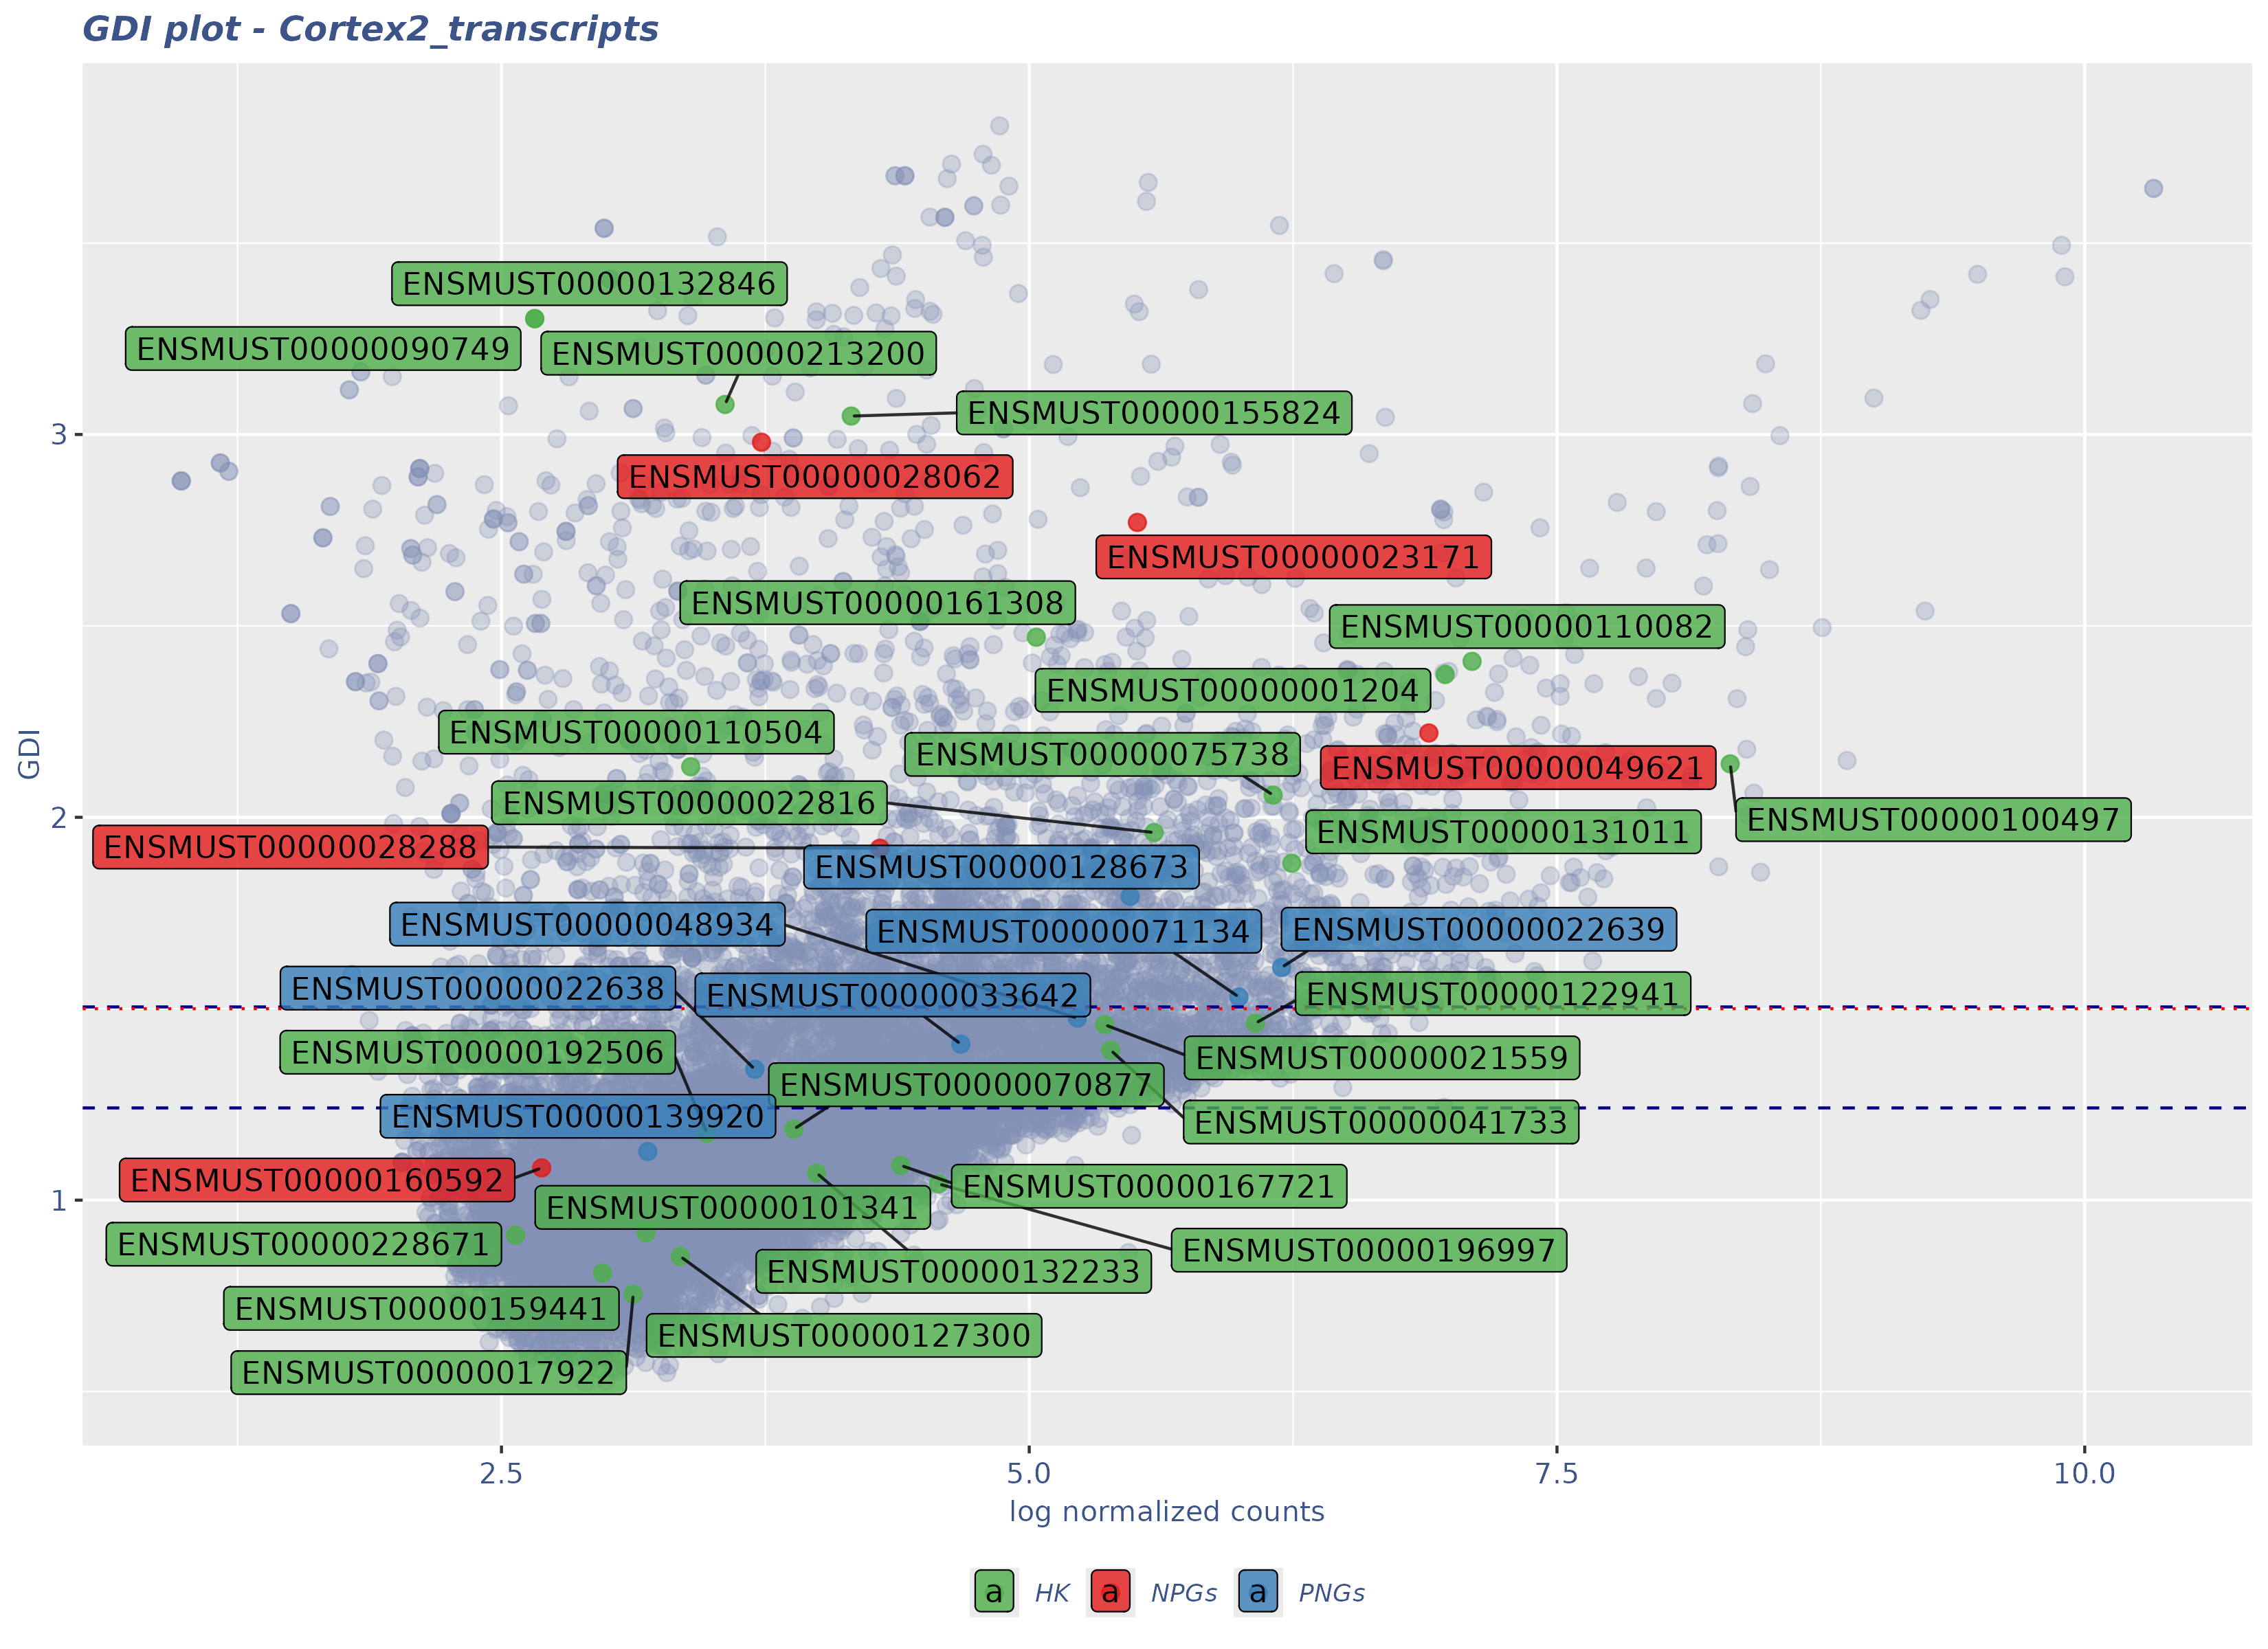
\includegraphics[width=0.8\textwidth]{GDI_transcript_plot_markers.png}
    \caption{Grafico GDI del dataset murino raggruppato sui conteggi a livello di trascritto (11 cluster). La netta separazione spaziale indica firme isoforma-specifiche robuste nonostante i dati sparsi.}
    \label{fig:gditranscript}
\end{figure}

\subsection*{Confronto tra struttura genica e struttura dei trascritti}

La Figura~\ref{fig:gdi_genes} mostra le stesse cellule raggruppate usando i conteggi genici standard (15 cluster). La diversa risoluzione dei cluster---gruppi più numerosi ma più piccoli rispetto al clustering sui trascritti---suggerisce che l'aggregazione ai geni perde struttura a grana fine. Questa differenza conta per la DTU: se i segnali specifici delle isoforme guidano l'identità cellulare, la media a livello genico li oscurerebbe.

Il confronto rivela anche quali cellule sono più influenzate dalla scelta di clustering. Le cellule vicine ai confini tra cluster in un metodo ma interne ai cluster nell'altro rappresentano casi ambigui in cui la classificazione dipende dalla risoluzione. Questi casi limite possono spiegare perché alcuni eventi DTU compaiono solo con specifiche strategie di clustering (discusso più avanti).

\begin{figure}[htbp]
    \centering
    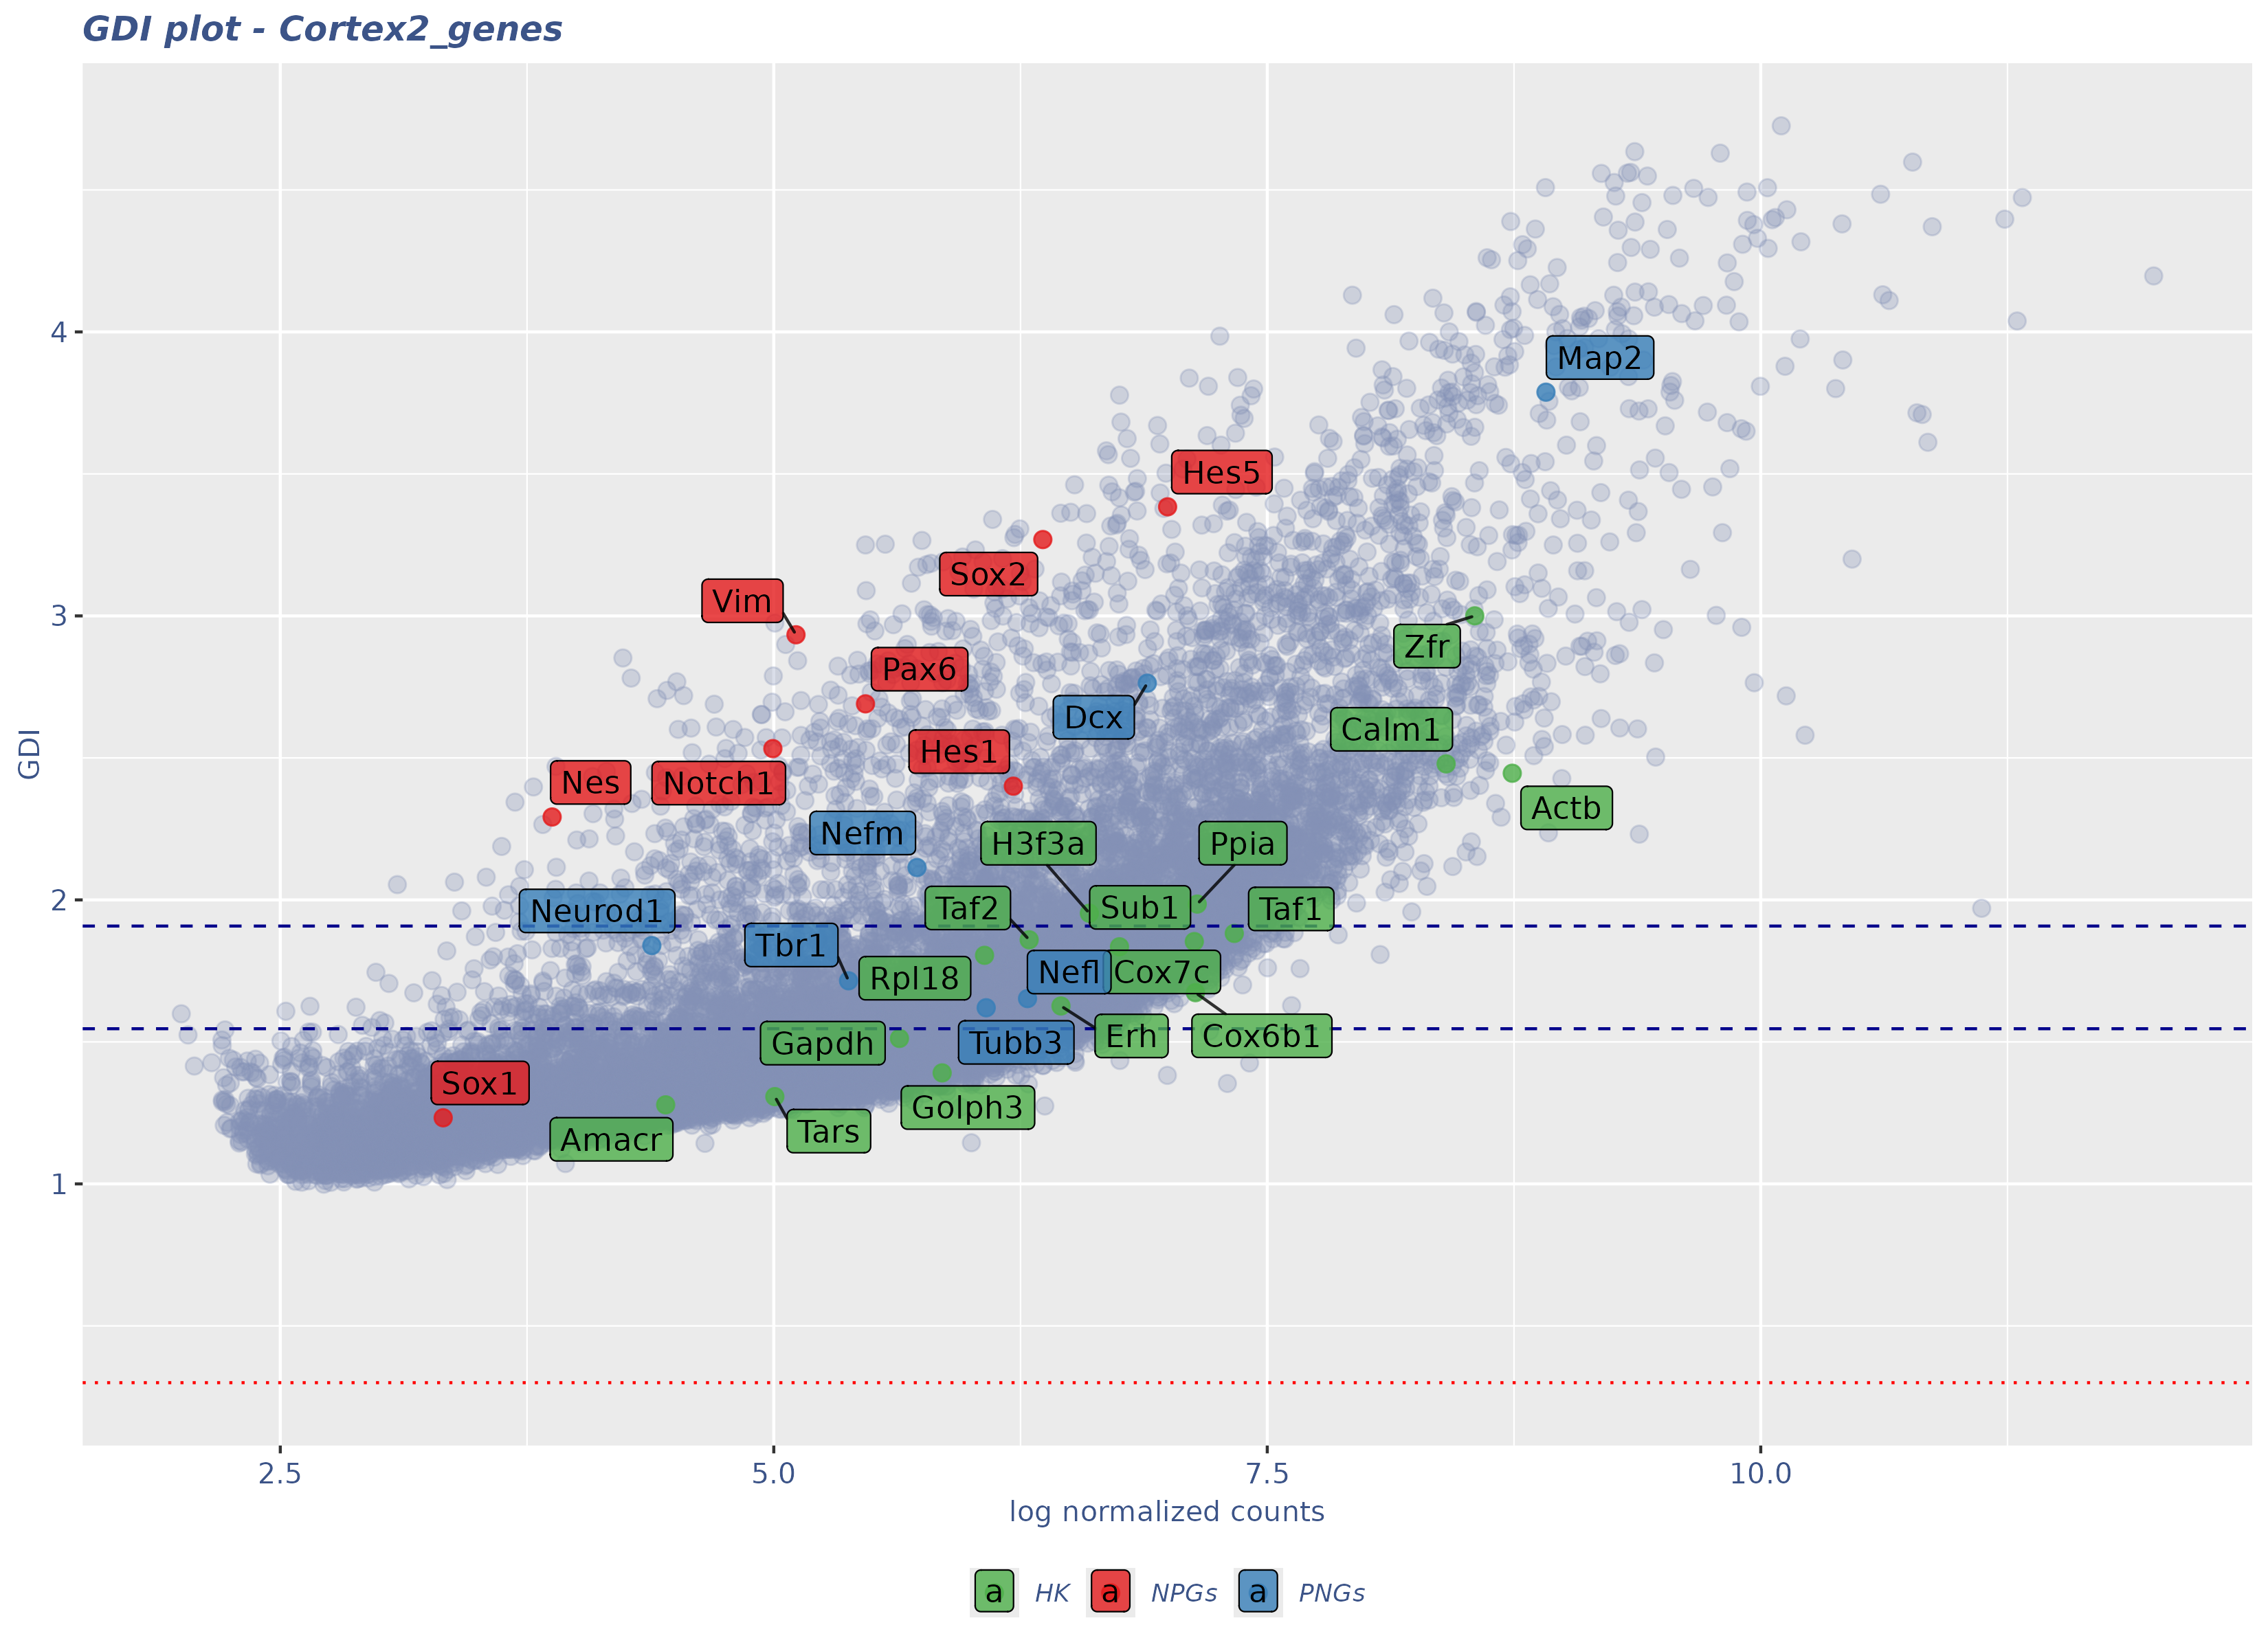
\includegraphics[width=0.8\textwidth]{GDI_genes_plot_markers.png}
    \caption{Grafico GDI del dataset murino raggruppato sui conteggi a livello genico (15 cluster). La diversa risoluzione rispetto al clustering sui trascritti suggerisce che l'aggregazione perde struttura a grana fine.}
    \label{fig:gdi_genes}
\end{figure}

Queste analisi GDI stabiliscono che entrambi gli approcci di clustering catturano segnale biologico reale, ma con sensibilità diversa alla sottostruttura cellulare. Si passa ora alla domanda principale: questa differenza strutturale si traduce in un rilevamento DTU diverso?

\section{Confronto tra clustering a livello genico e a livello di trascritto}\label{sec:clustering-comparison}

Per quantificare quanto i due clustering divergano, è stata costruita una matrice di confusione sulle 4.077 cellule comuni presenti in entrambe le analisi.

\begin{figure}[htbp]
    \centering
    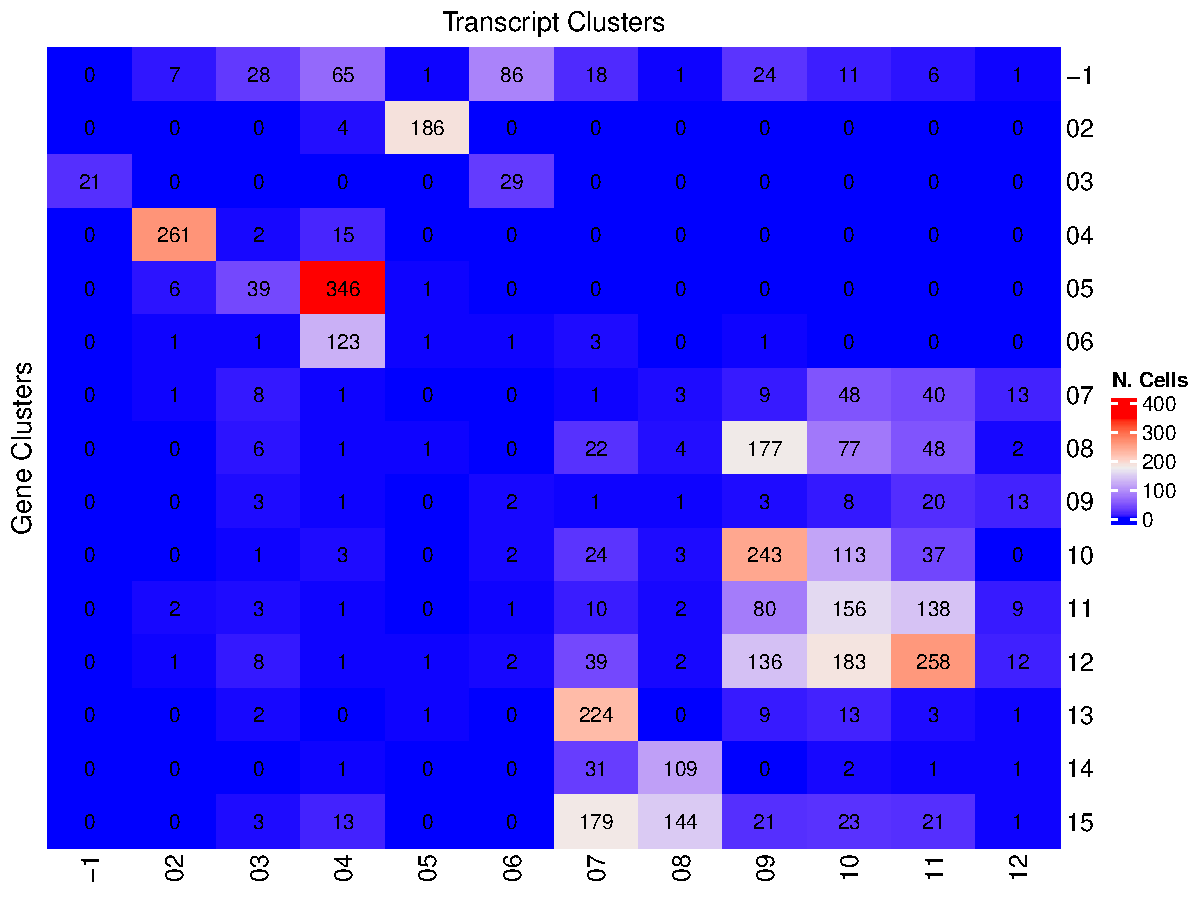
\includegraphics[width=0.8\textwidth]{heatmap_genes_vs_transcripts.pdf}
    \caption{Matrice di confusione che confronta le assegnazioni a livello di trascritto (11 cluster) e a livello genico (15 cluster) per le 4.077 cellule comuni del dataset murino. La dominanza della diagonale indica una sovrapposizione sostanziale; le voci fuori diagonale rivelano pattern sistematici di suddivisione e fusione.}
    \label{fig:confusion-matrix}
\end{figure}

La Figura~\ref{fig:confusion-matrix} mostra la heatmap della matrice di confusione. Emergono diversi pattern:
\begin{itemize}
    \item \textbf{Dominanza della diagonale}: la maggior parte delle cellule riceve assegnazioni coerenti nei due metodi, il che conferma che nessuno dei due produce cluster casuali.
    
    \item \textbf{Suddivisione sistematica}: diversi cluster a livello di trascritto corrispondono a sotto-regioni di un singolo cluster genico. Per esempio, il cluster 4 dei trascritti si separa dal più ampio cluster genico 7, suggerendo una variazione isoformica all'interno di ciò che appare omogeneo alla risoluzione genica.
    
    \item \textbf{Fusione selettiva}: viceversa, alcuni cluster adiacenti a livello di trascritto si fondono nell'analisi genica, indicando che le loro differenze dipendono da pattern di espressione specifici delle isoforme anziché dall'attività trascrizionale complessiva.
\end{itemize}

L'interpretazione è che il clustering a livello di trascritto rivela una sottostruttura cellulare invisibile all'aggregazione genica. È esattamente il regime in cui il rilevamento DTU dovrebbe aggiungere valore: se gli switch di isoforma distinguono stati cellulari che i soli geni non separano, i metodi isoform-aware catturano segnali biologicamente rilevanti.

Questo solleva però una domanda critica: gli eventi DTU rilevati sono robusti tra strategie di clustering, o dipendono interamente da come le cellule vengono partizionate? La questione è affrontata più avanti.

\section{Risultato principale: rilevamento della DTU}\label{sec:dtu-results}
\textit{(Questa sezione presenta il contributo principale di questa tesi---l'applicazione di COTAN al rilevamento DTU a livello di trascritto.)}

L'algoritmo della Sezione~\ref{sec:methods-dtu-algorithm} è stato applicato sia al dataset umano sia a quello murino, filtrando per coppie di isoforme mutuamente esclusive con preferenza bidirezionale tra cluster (soglia $\tau$ come specificato). I risultati dimostrano che le statistiche su tabelle di contingenza possono recuperare pattern di esclusività all'interno di un gene anche in dati sparsi $3'$-biased.

\subsection*{Risultati sul dataset umano (Arigoni)}\label{sec:results-human}

La miscela di linee cellulari umane ha fornito una validazione contro biologia nota. Dopo la soglia a $\tau = 0.2$ sono stati identificati:
\begin{itemize}
    \item \textbf{430 geni con coppie di isoforme significativamente mutuamente esclusive} ($p < 0.05$)
    \item \textbf{21 candidati DTU su 9 geni} che superano la soglia di contrasto bidirezionale
\end{itemize}

Il valore di $\tau$ più alto riflette cluster di linee cellulari ben definiti e ben separati, che consentono un filtraggio più severo per ottenere chiamate sicure.

Risultati rappresentativi:
\begin{enumerate}
    \item \textbf{TPM1 (tropomiosina 1)}: più isoforme mostrano preferenze opposte tra le linee cellulari. L'isoforma A è arricchita in PC9 e DV90; l'isoforma B domina in A549 e HCC78.
    
    \item \textbf{RPL10, RPS24 (proteine ribosomiali)}: segnali DTU inattesi nei geni ribosomiali suggeriscono una regolazione della traduzione specifica per tipo cellulare---coerente con l'eterogeneità della composizione ribosomiale alla base di una traduzione specializzata \cite{xue2012specialized}.
\end{enumerate}

L'elenco finale di candidati relativamente ridotto (9 geni) riflette il disegno conservativo dell'algoritmo: richiedere sia l'\gls{mutualExclusivity} sia il contrasto bidirezionale elimina le associazioni spurie.

\subsection*{Risultati sul dataset murino (Ding)}\label{sec:results-mouse}

Per il tessuto cerebrale murino è stata applicata una soglia più bassa ($\tau = 0.05$) per catturare transizioni più sottili lungo le traiettorie di differenziazione:
\begin{itemize}
    \item \textbf{14 geni con coppie significative}
    \item \textbf{46 candidati DTU su 8 geni} dopo il filtraggio sul contrasto
\end{itemize}

Il numero maggiore di candidati nonostante meno coppie significative iniziali suggerisce che il tessuto cerebrale murino mostri pattern di \gls{isoformSwitch} più graduali, anziché switch netti come quelli tra linee cellulari.

Risultati rappresentativi:
\begin{enumerate}
    \item \textbf{Meg3 (maternally expressed gene 3)}: RNA lungo non codificante\defn{RNA lungo non codificante (lncRNA)}{Una lunga molecola di RNA che non codifica una proteina ma regola l'espressione genica, lo splicing e lo sviluppo.} con un ruolo documentato nella differenziazione neuronale. L'isoforma A domina nei primi cluster progenitori; l'isoforma B è arricchita nei cluster di neuroni differenziati, uno switch che segue la traiettoria di differenziazione anziché uno stato binario netto.
    
    \item \textbf{Malat1 (metastasis-associated lung adenocarcinoma transcript 1)}: un altro lncRNA altamente conservato coinvolto nella regolazione dello splicing. Mostra preferenze di isoforma specifiche per cluster, coerenti con l'uso alternativo dell'isoforma 3$'$ documentato per questo locus \cite{ghanam2023malat1}.

    \item \textbf{Srrm2 (serine/arginine-rich splicing factor 2)}: codifica una componente centrale dello spliceosoma\defn{Spliceosoma}{La macchina molecolare che rimuove gli introni e unisce gli esoni durante lo splicing.}. La sua stessa DTU suggerisce una regolazione a feedback---lo splicing alternativo dei fattori di splicing è un meccanismo noto per modulare il panorama delle isoforme tra stati cellulari.

    \item \textbf{Ttc14 (tetratricopeptide repeat domain 14)}: candidato nuovo, senza letteratura DTU precedente. Richiede una \gls{orthogonalValidation} per confermarne il significato biologico.
\end{enumerate}

Questi hit su lncRNA (Meg3, Malat1) sono particolarmente incoraggianti perché si confermano rispetto a biologia nota nonostante il vincolo del bias 3'---dimostrando che COTAN a livello di trascritto può recuperare segnali reali anche in condizioni difficili.


\subsection*{Analisi di robustezza: eventi condivisi ed esclusivi}\label{sec:robustness}

Il rilevamento DTU è stato rieseguito usando le etichette di cluster derivate dai geni sulla stessa matrice di trascritti, poi gli elenchi di eventi sono stati confrontati tra le due strategie di clustering:

\begin{table}[htbp]
\centering
\begin{tabular}{lcc}
    \toprule
    & \textbf{Clustering sui trascritti} & \textbf{Clustering sui geni} \\
    \midrule
    Coppie DTU totali rilevate & 46 & 46 \\
    \bottomrule
\end{tabular}
\caption{Sovrapposizione degli eventi DTU tra le strategie di clustering (dataset murino). Totali uguali ma composizione diversa rivelano i pattern di robustezza.}
\label{tab:dtu-robustness}
\end{table}

Ripartizione della composizione degli eventi:
\begin{itemize}
    \item \textbf{Eventi condivisi}: la maggioranza delle coppie è rilevata da entrambi i metodi, tra cui Meg3 e Malat1---si tratta di segnali forti che sopravvivono indipendentemente dallo schema di partizione.
    
    \item \textbf{Esclusivi dei trascritti (3 coppie)}: gli switch di isoforma di Srrm2 e Ttc14 compaiono solo con i cluster derivati dai trascritti. Riflettono probabilmente transizioni sottili che richiedono una risoluzione fine della popolazione per essere rilevate.

    \item \textbf{Esclusivi dei geni (4 coppie)}: Snrnp70, Lrrc7, Zfp941 e una specifica coppia di Meg3 sono rilevati solo con il clustering a livello genico. Possono rappresentare segnali più deboli che beneficiano della potenza statistica aggregata.
\end{itemize}

L'interpretazione:
\begin{enumerate}
    \item I segnali DTU più forti (grande dimensione dell'effetto) sopravvivono a entrambi gli approcci, il che convalida la funzionalità di base dell'algoritmo.
    
    \item Gli switch sottili dipendono dalla risoluzione del clustering: il livello di trascritto cattura stati specifici delle isoforme, il livello genico fornisce potenza per i trascritti a bassa abbondanza.
    
    \item Nessun approccio domina in modo universale. La scelta dovrebbe dipendere dalla domanda biologica: sottostruttura a grana fine o robustezza statistica.
\end{enumerate}

Questa analisi di robustezza conferma che, mentre i segnali più forti sono indipendenti dal clustering, gli switch di isoforma sottili si rivelano solo con schemi di partizione adeguati. La scelta della strategia di clustering non è soltanto tecnica: determina quale biologia diventa visibile.

\section*{Nota sulla sensibilità ai parametri}

Il parametro di soglia $\tau$ è stato tarato empiricamente per produrre un numero di candidati biologicamente ragionevole (20--100 eventi validabili). Uno script di taratura dedicato è incluso nel repository GitHub, e lavori futuri potranno affinare questa scelta con un controllo del tasso di falsi positivi basato su permutazioni\defn{Test di permutazione}{Una procedura che rimescola le etichette per costruire una distribuzione nulla empirica, sostituendo una soglia arbitraria.} o con validazione incrociata su dataset ortogonali.

\section{Discussione}\label{sec:discussion}

I risultati vengono ora collocati nel più ampio contesto metodologico e biologico.

\subsection*{Interpretazione dei risultati principali}

Dai risultati emergono tre conclusioni centrali:
\begin{enumerate}
    \item \textbf{Fattibilità confermata}: il framework a tabelle di contingenza di COTAN rileva con successo la DTU in dati sparsi $3'$-biased. Questo ne estende l'applicabilità oltre la co-espressione a livello genico, fino all'analisi a risoluzione di isoforma.

    \item \textbf{Plausibilità biologica convalidata}: i candidati principali (Meg3, Malat1, TPM1) sono coerenti con biologia nota---switch di lncRNA nella neurogenesi e regolazione delle proteine ribosomiali. Questo suggerisce che l'algoritmo recuperi segnale reale anziché artefatti tecnici.

    \item \textbf{Il clustering conta}: la divergenza tra le chiamate DTU a livello di trascritto e a livello genico mostra che gli switch di isoforma possono distinguere sottostati cellulari invisibili ai conteggi aggregati. Un clustering a grana fine rende possibile il rilevamento di transizioni sottili.
\end{enumerate}

La convergenza tra dataset (linee cellulari umane e cervello murino) rafforza la fiducia nel metodo: funziona in contesti biologici diversi, non solo in un singolo caso favorevole.

\subsection*{Limiti e avvertenze}

Nonostante i risultati incoraggianti, alcuni vincoli ne temperano l'interpretazione:
\begin{itemize}
    \item \textbf{Invisibilità dovuta al bias $3'$}: gli eventi di splicing alternativo che avvengono nelle regioni centrali del trascritto restano non rilevabili quando si sequenziano solo le \gls{threePrimeEnd}. I candidati DTU trovati rappresentano un sottoinsieme---quelli in cui le isoforme differiscono negli esoni terminali o alle estremità 3'.

    \item \textbf{Effetti dell'arrotondamento EM}: le assegnazioni frazionarie dell'EM sono state arrotondate a interi per compatibilità con COTAN. Le isoforme a bassa abbondanza, con conteggi frazionari piccoli, possono risultare distorte da questa discretizzazione, con la possibile introduzione di falsi negativi o l'alterazione dei valori di contrasto.

    \item \textbf{Sensibilità alla soglia}: la scelta di $\tau$ manca di un fondamento statistico formale. La taratura empirica ha prodotto numeri di candidati ragionevoli, ma una distribuzione nulla basata su permutazioni fornirebbe $p$-value calibrati al posto di soglie arbitrarie.

    \item \textbf{Assenza di validazione ortogonale}: senza sequenziamento long-read o conferma mirata tramite RT-PCR\defn{RT-PCR}{Reverse-transcription polymerase chain reaction: una tecnica di laboratorio che conferma sperimentalmente la presenza di una specifica isoforma, usata come verifica ortogonale delle chiamate DTU computazionali.}, i tassi di falsi positivi restano stimati a partire dalla coerenza interna (eventi condivisi ed esclusivi) anziché da una verità di riferimento.

Questa è una limitazione comune agli studi DTU computazionali, ma resta critica per le affermazioni biologiche.
\end{itemize}

Questi limiti indicano direzioni concrete di miglioramento: read più lunghi per una copertura completa delle isoforme, una migliore gestione dell'EM tramite metodi a conteggi frazionari, una calibrazione formale delle soglie e una validazione sperimentale dei candidati principali.

\subsection*{Direzioni future: estendere COTAN all'analisi dei trascritti}

Il framework qui stabilito apre diverse vie di estensione metodologica:
\begin{enumerate}
    \item \textbf{Integrazione con dati long-read}: combinare la profondità short-read (migliaia di cellule) con l'annotazione delle isoforme da PacBio/Nanopore\defn{Sequenziamento long-read (PacBio, Oxford Nanopore)}{Tecnologie di sequenziamento che producono read full-length dei trascritti, fornendo un'annotazione completa delle isoforme non disponibile dai read brevi $3'$-biased.} ancorerebbe le chiamate DTU a sequenze complete dei trascritti.

Questo approccio ibrido potrebbe validare le previsioni computazionali mantenendo la scalabilità a campioni di dimensione di popolazione.

    \item \textbf{Analisi sensibile alla traiettoria}: il clustering attuale assume popolazioni cellulari discrete, ma la differenziazione è continua. Modellare le proporzioni delle isoforme lungo traiettorie di pseudotempo\defn{Pseudotempo}{Un ordinamento monodimensionale delle cellule lungo una traiettoria continua di sviluppo o differenziazione, che cattura transizioni graduali anziché popolazioni discrete.} (ad esempio adattando il framework di COTAN alla regressione anziché al confronto categoriale) potrebbe rivelare pattern dinamici di switch durante le transizioni.

    \item \textbf{Estensione all'espressione allele-specifica}: l'approccio a tabelle di contingenza di COTAN si estende naturalmente a varianti fase. Rilevare un uso delle isoforme sbilanciato per allele collegherebbe la genetica regolatoria (eQTL, sQTL)\defn{eQTL / sQTL}{Varianti genomiche che influenzano misurabilmente l'espressione genica (eQTL) o lo splicing e l'uso delle isoforme (sQTL); collegarle agli switch di isoforma a singola cellula connette la genetica di popolazione con la regolazione.} agli esiti dello splicing nelle singole cellule---ponendo un ponte tra genomica di popolazione e regolazione dei trascritti.

    \item \textbf{Benchmark contro strumenti DTU bulk}: un confronto sistematico con rMATS, SUPPA2 e DRIMSeq \cite{love2018swimming, draper2025selecting} su pseudo-bulk appaiati collocherebbe sensibilità e specificità nel giusto contesto. Questo benchmark potrebbe individuare i regimi in cui i metodi a singola cellula aggiungono valore unico e quelli in cui l'aggregazione è sufficiente.
\end{enumerate}

Queste estensioni restano oltre lo scopo di questa tesi, ma dimostrano che COTAN a livello di trascritto non è una soluzione definitiva: esso stabilisce piuttosto una prova di concetto per un'analisi delle isoforme robusta alla sparsità nelle singole cellule. La flessibilità del framework suggerisce ulteriori adattamenti man mano che emergono nuovi tipi di dati e nuove domande biologiche.

\section*{Sintesi}

Questo capitolo ha presentato i risultati del rilevamento DTU dall'applicazione di COTAN a dati scRNA-seq a livello di trascritto. Risultati principali:
\begin{itemize}
    \item 21 candidati DTU (umano) e 46 candidati DTU (topo) identificati con confidenza statistica.
    \item I principali hit (Meg3, Malat1, TPM1) sono coerenti con biologia nota nonostante i vincoli del bias 3' \cite{ghanam2023malat1, xue2012specialized}.
    \item La strategia di clustering influenza quali eventi vengono rilevati: il livello di trascritto rivela struttura a grana fine, il livello genico fornisce robustezza per i segnali deboli.
\end{itemize}

Il capitolo successivo riassume queste conclusioni e delinea i contributi più ampi della tesi alla genomica computazionale.

\chapter{Conclusioni}

Questa tesi ha stabilito che il quadro a tabelle di contingenza di COTAN, robusto alla sparsità, può essere esteso all'analisi a livello di trascritto, recuperando pattern di esclusività all'interno di un gene che indicano un uso differenziale dei trascritti (DTU) a partire da dati sparsi di \gls{rnaSeq} a singola cellula $3'$-biased. L'intuizione chiave---che i pattern di zeri portano segnale affidabile anche in matrici estremamente rade---si trasferisce con successo dalla co-espressione genica al rilevamento dell'\gls{mutualExclusivity} tra isoforme.

\section{Sintesi dei risultati}

Applicato ai due dataset a goccia, il quadro adattato ha restituito segnale rilevabile in entrambi: 430 geni umani portavano una coppia di isoforme significativamente mutuamente esclusive, con 21 candidati che superavano il filtro a contrasto bidirezionale, e 46 candidati murini che passavano alla soglia più bassa. Le chiamate più forti---TPM1 nella miscela di linee cellulari, Meg3 e Malat1 nella corteccia murina---sono coerenti con la biologia delle isoforme documentata \cite{ghanam2023malat1, xue2012specialized}, e la maggior parte è sopravvissuta allo scambio della strategia di clustering, quindi il segnale non dipende da un particolare schema di partizione.

\section{Implicazioni più ampie}

Questo lavoro ha implicazioni in tre ambiti:

\textbf{Per la genomica computazionale}: il successo delle statistiche a tabelle di contingenza a risoluzione di trascritto dimostra che la sparsità non deve essere trattata come un problema da superare (tramite imputazione o trasformazione logaritmica), ma piuttosto da modellare direttamente. Questa filosofia può estendersi ad altre sfide a singola cellula---espressione allele-specifica, co-occorrenza di picchi di accessibilità della cromatina e integrazione multi-modale.

\textbf{Per la biologia delle isoforme}: rilevare la DTU nei dati $3'$-biased apre nuove opportunità di analisi per dataset su larga scala già esistenti (per esempio Human Cell Atlas e Tabula Sapiens\defn{Human Cell Atlas / Tabula Sapiens}{Grandi atlanti di riferimento internazionali di trascrittomi a singola cellula in tessuti umani, basati su dati a goccia $3'$-biased e quindi chiusi alle domande a livello di isoforma.}) che erano precedentemente preclusi alle domande a livello di isoforma. Sebbene la sensibilità resti limitata rispetto ai protocolli full-length, il compromesso tra numero di cellule e copertura può favorire i metodi a goccia quando la potenza statistica di migliaia di cellule supera la profondità per cellula.

\textbf{Per lo sviluppo del framework COTAN}: questa tesi conferma che i principi di progettazione di COTAN---la modellazione diretta dei conteggi nulli e la calibrazione $\chi^2$ dei $p$-value su grandi $N$---si generalizzano oltre l'analisi a livello genico. Estensioni future ad altre modalità a singola cellula (co-occorrenza di picchi ATAC-seq\defn{ATAC-seq}{Assay for Transposase-Accessible Chromatin: mappa le regioni del genoma in cui la cromatina è aperta, indicando attività regolatoria.} e correlazioni di abbondanza proteica in CITE-seq\defn{CITE-seq}{Un protocollo che misura simultaneamente RNA e proteine di superficie nelle stesse singole cellule, abilitando l'analisi multi-modale.}) appaiono praticabili.

\section{Limiti e lavoro futuro}

I vincoli su questi risultati---invisibilità dovuta al bias $3'$, assenza di validazione ortogonale, soglia euristica $\tau$ e arrotondamento dell'EM---sono esposti insieme alle direzioni che aprono nella Sezione~\ref{sec:discussion}. Lo stesso compromesso di fondo li governa tutti e quattro: la sensibilità si compra con le cellule anziché con la copertura, quindi il valore del metodo cresce con i dataset.

Un quantificatore più recente punta nella stessa direzione. SCALPEL\cite{ake2025scalpel} costruisce la matrice di trascritti da dati $3'$-based standard seguendo una via diversa dal passo EM usato qui, e i suoi autori riportano sensibilità superiore e un recupero più fedele delle reali proporzioni di isoforme rispetto agli strumenti esistenti, con validazione sperimentale. Sostituirlo a \texttt{parsimony-em} verificherebbe se le chiamate di DTU a valle diventano più nitide, il che lo rende un'estensione naturale di questo quadro.

\section*{Considerazioni finali}

Questa tesi dimostra che COTAN a livello di trascritto può rivelare programmi regolatori nascosti alle analisi centrate sui geni. Il quadro a tabelle di contingenza fornisce un approccio rigoroso all'analisi di dati sparsi---un approccio che rispetta il processo di misura reale anziché imporre trasformazioni pensate per dati densi e distribuiti normalmente.

Il cammino futuro richiede validazione ortogonale e le tecnologie complementari indicate nella Sezione~\ref{sec:discussion} perché i metodi isoform-aware a singola cellula passino dalla prova di fattibilità alla pratica standard.

Il quadro stabilito qui fornisce una base per quel lavoro futuro---combinando rigore metodologico (statistiche a tabelle di contingenza), riproducibilità computazionale (pipeline Nextflow documentata) e validazione biologica (allineamento con switch di isoforma noti). Che venga applicato alla neurogenesi, all'evoluzione del cancro o alla biologia dello sviluppo, la domanda di fondo resta la stessa: \textit{quali trascritti esprimono le cellule, e come cambia questa scelta tra condizioni diverse?}


% Bibliography (global, after all chapters)
\cleardoublepage
\addcontentsline{toc}{chapter}{Bibliografia}
\bibliographystyle{unsrt}
\bibliography{bib/riferimenti}

% Appendix (optional)
\appendix
\chapter{Dati Supplementari}
\thispagestyle{empty}
\section{Risultati DTU completi (dataset Arigoni e Ding)}

\pagestyle{empty}

% --- TABELLA 1: ARRIGONI ---
\begin{landscape}
\begingroup
\footnotesize
\setlength{\tabcolsep}{4.5pt}
\begin{longtable}{@{} l l l >{\raggedright\arraybackslash}p{3.4cm} >{\raggedright\arraybackslash}p{3.4cm} r r r r @{}}
\caption{Eventi DTU significativi nel dataset umano (Arigoni 2024), con arricchimento per cluster e contrasti massimi.\label{tab:arrigoni_landscape}}\\
\toprule
\textbf{Gene} & \textbf{Tr.~A} & \textbf{Tr.~B} & \textbf{Cluster A} & \textbf{Cluster B} & \textbf{$\Delta$ A} & \textbf{$\Delta$ B} & \textbf{COEX} & \textbf{$p$-value} \\
\midrule
\endfirsthead
\toprule
\textbf{Gene} & \textbf{Tr.~A} & \textbf{Tr.~B} & \textbf{Cluster A} & \textbf{Cluster B} & \textbf{$\Delta$ A} & \textbf{$\Delta$ B} & \textbf{COEX} & \textbf{$p$-value} \\
\midrule
\endhead
\midrule
\multicolumn{9}{r}{\textit{Continua nella pagina successiva}} \\
\endfoot
\bottomrule
\endlastfoot
TPM1   & ENST00000334895 & ENST00000358278 & DV90, HCC78, HTB178 & A549, CCL-185-IG & 0.33 & 0.61 & $-0.101$ & $7.72 \times 10^{-67}$ \\
RPL10  & ENST00000406022 & ENST00000458500 & A549 & HCC78, PC9 & 0.22 & 0.46 & $-0.086$ & $2.78 \times 10^{-49}$ \\
RPL10  & ENST00000458500 & ENST00000491035 & HCC78, PC9 & A549, PBMCs & 0.46 & 0.25 & $-0.084$ & $6.41 \times 10^{-47}$ \\
TPM1   & ENST00000404484 & ENST00000651344 & HCC78, HTB178 & A549, CCL-185-IG & 0.27 & 0.37 & $-0.074$ & $1.15 \times 10^{-36}$ \\
TPM1   & ENST00000317516 & ENST00000651344 & HCC78, HTB178 & A549, CCL-185-IG & 0.28 & 0.36 & $-0.068$ & $4.41 \times 10^{-31}$ \\
RPS24  & ENST00000360830 & ENST00000465692 & DV90, HCC78 & CCL-185-IG, HTB178, PBMCs & 0.28 & 0.30 & $-0.051$ & $1.76 \times 10^{-18}$ \\
TPM1   & ENST00000288398 & ENST00000334895 & A549, CCL-185-IG & HTB178 & 0.30 & 0.21 & $-0.047$ & $1.13 \times 10^{-15}$ \\
TPM1   & ENST00000560959 & ENST00000651344 & HCC78, HTB178 & A549, CCL-185-IG & 0.22 & 0.32 & $-0.044$ & $8.17 \times 10^{-14}$ \\
RPS24  & ENST00000360830 & ENST00000482069 & DV90, HCC78 & CCL-185-IG, HTB178, PBMCs & 0.28 & 0.28 & $-0.040$ & $8.15 \times 10^{-12}$ \\
TPM1   & ENST00000334895 & ENST00000651344 & DV90, HCC78, HTB178 & A549, CCL-185-IG & 0.28 & 0.44 & $-0.040$ & $8.76 \times 10^{-12}$ \\
DSTN   & ENST00000449141 & ENST00000474024 & HTB178 & CCL-185-IG & 0.28 & 0.22 & $-0.039$ & $3.70 \times 10^{-11}$ \\
SAT1   & ENST00000379253 & ENST00000462639 & A549 & PC9 & 0.26 & 0.27 & $-0.038$ & $6.62 \times 10^{-11}$ \\
TPM4   & ENST00000645471 & ENST00000646974 & CCL-185-IG & HCC78 & 0.32 & 0.39 & $-0.034$ & $5.27 \times 10^{-09}$ \\
SAT1   & ENST00000379251 & ENST00000462639 & A549 & PC9 & 0.22 & 0.21 & $-0.031$ & $7.47 \times 10^{-08}$ \\
SAT1   & ENST00000379270 & ENST00000487713 & A549 & PC9 & 0.25 & 0.25 & $-0.031$ & $9.35 \times 10^{-08}$ \\
RPL35A & ENST00000429437 & ENST00000642387 & PC9 & PBMCs & 0.21 & 0.22 & $-0.031$ & $1.26 \times 10^{-07}$ \\
TPM1   & ENST00000558544 & ENST00000651344 & HCC78, HTB178 & A549, CCL-185-IG & 0.23 & 0.33 & $-0.019$ & $1.04 \times 10^{-03}$ \\
TPM1   & ENST00000358278 & ENST00000558868 & A549, CCL-185-IG & CRL5868, DV90, HCC78, HTB178 & 0.52 & 0.27 & $-0.018$ & $1.96 \times 10^{-03}$ \\
SNHG5  & ENST00000654795 & ENST00000664396 & CCL-185-IG & PC9 & 0.23 & 0.28 & $-0.018$ & $2.37 \times 10^{-03}$ \\
RPS8   & ENST00000372209 & ENST00000485390 & PC9 & PBMCs & 0.21 & 0.29 & $-0.017$ & $4.19 \times 10^{-03}$ \\
TPM1   & ENST00000317516 & ENST00000358278 & DV90, HCC78, HTB178 & A549, CCL-185-IG & 0.33 & 0.54 & $-0.012$ & $4.03 \times 10^{-02}$ \\
\end{longtable}
\endgroup
\end{landscape}


% --- TABELLA 2: DING CONDIVISI ---
\begin{landscape}
\begingroup
\footnotesize
\setlength{\tabcolsep}{4.5pt}
\begin{longtable}{@{} l l l >{\raggedright\arraybackslash}p{3.4cm} >{\raggedright\arraybackslash}p{3.4cm} r r r r @{}}
\caption{Eventi DTU condivisi rilevati da entrambi i metodi di clustering (dataset Ding), con tipi cellulari e contrasti.\label{tab:shared_landscape}}\\
\toprule
\textbf{Gene} & \textbf{Tr.~A} & \textbf{Tr.~B} & \textbf{Cluster A} & \textbf{Cluster B} & \textbf{$\Delta$ A} & \textbf{$\Delta$ B} & \textbf{COEX} & \textbf{$p$-value} \\
\midrule
\endfirsthead
\toprule
\textbf{Gene} & \textbf{Tr.~A} & \textbf{Tr.~B} & \textbf{Cluster A} & \textbf{Cluster B} & \textbf{$\Delta$ A} & \textbf{$\Delta$ B} & \textbf{COEX} & \textbf{$p$-value} \\
\midrule
\endhead
\midrule
\multicolumn{9}{r}{\textit{Continua nella pagina successiva}} \\
\endfoot
\bottomrule
\endlastfoot
Meg3   & ENSMUST00000146701 & ENSMUST00000246047 & 07, 08, 09, 10, 11, 12 & $-1$, 02, 03, 04, 05, 06 & 0.28 & 0.66 & $-0.174$ & $1.58 \times 10^{-28}$ \\
Meg3   & ENSMUST00000129245 & ENSMUST00000146701 & $-1$, 02, 03, 04, 05, 06 & 07, 08, 09, 10, 11, 12 & 0.63 & 0.28 & $-0.160$ & $1.65 \times 10^{-24}$ \\
Malat1 & ENSMUST00000173499 & ENSMUST00000245771 & 08, 10, 11, 12 & 02, 04, 05, 06 & 0.27 & 0.29 & $-0.104$ & $2.91 \times 10^{-11}$ \\
Malat1 & ENSMUST00000173499 & ENSMUST00000245150 & 08, 09, 10, 11, 12 & $-1$, 02, 04, 05, 06 & 0.17 & 0.29 & $-0.073$ & $3.30 \times 10^{-06}$ \\
Meg3   & ENSMUST00000129245 & ENSMUST00000247387 & 02, 04, 05, 06 & 11, 12 & 0.34 & 0.29 & $-0.043$ & $5.70 \times 10^{-03}$ \\
Meg3   & ENSMUST00000129245 & ENSMUST00000246553 & 02, 04, 05, 06 & 11, 12 & 0.34 & 0.29 & $-0.042$ & $6.88 \times 10^{-03}$ \\
Meg3   & ENSMUST00000129245 & ENSMUST00000245180 & 02, 04, 05, 06 & 11, 12 & 0.33 & 0.30 & $-0.042$ & $7.27 \times 10^{-03}$ \\
Meg3   & ENSMUST00000129245 & ENSMUST00000246499 & 02, 04, 05, 06 & 11, 12 & 0.33 & 0.29 & $-0.042$ & $7.40 \times 10^{-03}$ \\
Meg3   & ENSMUST00000246047 & ENSMUST00000247387 & 02, 04, 05, 06 & 11, 12 & 0.37 & 0.29 & $-0.042$ & $7.96 \times 10^{-03}$ \\
Meg3   & ENSMUST00000129245 & ENSMUST00000246427 & 02, 04, 05, 06 & 11, 12 & 0.33 & 0.29 & $-0.041$ & $8.84 \times 10^{-03}$ \\
Meg3   & ENSMUST00000246047 & ENSMUST00000246553 & 02, 04, 05, 06 & 11, 12 & 0.37 & 0.29 & $-0.041$ & $9.49 \times 10^{-03}$ \\
Meg3   & ENSMUST00000129245 & ENSMUST00000246700 & 02, 04, 05, 06 & 11, 12 & 0.33 & 0.29 & $-0.041$ & $9.51 \times 10^{-03}$ \\
Meg3   & ENSMUST00000245180 & ENSMUST00000246047 & 11, 12 & 02, 04, 05, 06 & 0.29 & 0.37 & $-0.041$ & $9.66 \times 10^{-03}$ \\
Meg3   & ENSMUST00000246047 & ENSMUST00000246499 & 02, 04, 05, 06 & 11, 12 & 0.36 & 0.29 & $-0.040$ & $9.79 \times 10^{-03}$ \\
Meg3   & ENSMUST00000129245 & ENSMUST00000143836 & 02, 04, 05, 06 & 11, 12 & 0.33 & 0.29 & $-0.040$ & $9.83 \times 10^{-03}$ \\
Meg3   & ENSMUST00000129245 & ENSMUST00000245980 & 02, 04, 05, 06 & 11, 12 & 0.33 & 0.29 & $-0.040$ & $1.04 \times 10^{-02}$ \\
Meg3   & ENSMUST00000246047 & ENSMUST00000246427 & 02, 04, 05, 06 & 11, 12 & 0.36 & 0.29 & $-0.040$ & $1.15 \times 10^{-02}$ \\
Meg3   & ENSMUST00000246047 & ENSMUST00000246700 & 02, 04, 05, 06 & 11, 12 & 0.36 & 0.29 & $-0.039$ & $1.24 \times 10^{-02}$ \\
Meg3   & ENSMUST00000129245 & ENSMUST00000247194 & 02, 04, 05, 06 & 11, 12 & 0.32 & 0.29 & $-0.039$ & $1.26 \times 10^{-02}$ \\
Meg3   & ENSMUST00000143836 & ENSMUST00000246047 & 11, 12 & 02, 04, 05, 06 & 0.28 & 0.36 & $-0.039$ & $1.27 \times 10^{-02}$ \\
Meg3   & ENSMUST00000245980 & ENSMUST00000246047 & 11, 12 & 02, 04, 05, 06 & 0.28 & 0.36 & $-0.039$ & $1.36 \times 10^{-02}$ \\
Meg3   & ENSMUST00000246047 & ENSMUST00000247194 & 02, 04, 05, 06 & 11, 12 & 0.36 & 0.28 & $-0.038$ & $1.60 \times 10^{-02}$ \\
Pde10a & ENSMUST00000141877 & ENSMUST00000233652 & 07 & 09, 10, 11 & 0.51 & 0.13 & $-0.037$ & $1.67 \times 10^{-02}$ \\
Meg3   & ENSMUST00000129245 & ENSMUST00000243087 & 02, 04, 05, 06 & 11, 12 & 0.32 & 0.24 & $-0.034$ & $3.21 \times 10^{-02}$ \\
Grin2b & ENSMUST00000053880 & ENSMUST00000125905 & 11 & 02, 04 & 0.10 & 0.10 & $-0.033$ & $3.39 \times 10^{-02}$ \\
Meg3   & ENSMUST00000129245 & ENSMUST00000246154 & 02, 04, 05, 06 & 11, 12 & 0.32 & 0.25 & $-0.033$ & $3.47 \times 10^{-02}$ \\
Meg3   & ENSMUST00000129245 & ENSMUST00000243937 & 02, 04, 05, 06 & 11, 12 & 0.31 & 0.25 & $-0.033$ & $3.79 \times 10^{-02}$ \\
Meg3   & ENSMUST00000243087 & ENSMUST00000246047 & 11, 12 & 02, 04, 05, 06 & 0.24 & 0.35 & $-0.032$ & $3.82 \times 10^{-02}$ \\
Meg3   & ENSMUST00000129245 & ENSMUST00000143847 & 02, 04, 05, 06 & 11, 12 & 0.31 & 0.24 & $-0.032$ & $3.98 \times 10^{-02}$ \\
Meg3   & ENSMUST00000129245 & ENSMUST00000247320 & 02, 04, 05, 06 & 11, 12 & 0.31 & 0.24 & $-0.032$ & $3.98 \times 10^{-02}$ \\
Meg3   & ENSMUST00000126289 & ENSMUST00000129245 & 11, 12 & 02, 04, 05, 06 & 0.25 & 0.31 & $-0.032$ & $4.08 \times 10^{-02}$ \\
Meg3   & ENSMUST00000246047 & ENSMUST00000246154 & 02, 04, 05, 06 & 11, 12 & 0.35 & 0.24 & $-0.032$ & $4.12 \times 10^{-02}$ \\
Meg3   & ENSMUST00000129245 & ENSMUST00000247335 & 02, 04, 05, 06 & 11, 12 & 0.31 & 0.25 & $-0.032$ & $4.19 \times 10^{-02}$ \\
Meg3   & ENSMUST00000243937 & ENSMUST00000246047 & 11, 12 & 02, 04, 05, 06 & 0.24 & 0.35 & $-0.031$ & $4.45 \times 10^{-02}$ \\
Meg3   & ENSMUST00000143847 & ENSMUST00000246047 & 11, 12 & 02, 04, 05, 06 & 0.24 & 0.35 & $-0.031$ & $4.66 \times 10^{-02}$ \\
Meg3   & ENSMUST00000246047 & ENSMUST00000247320 & 02, 04, 05, 06 & 11, 12 & 0.35 & 0.24 & $-0.031$ & $4.66 \times 10^{-02}$ \\
Meg3   & ENSMUST00000129245 & ENSMUST00000246462 & 02, 04, 05, 06 & 11, 12 & 0.31 & 0.24 & $-0.031$ & $4.73 \times 10^{-02}$ \\
Meg3   & ENSMUST00000126289 & ENSMUST00000246047 & 11, 12 & 02, 04, 05, 06 & 0.25 & 0.35 & $-0.031$ & $4.81 \times 10^{-02}$ \\
Meg3   & ENSMUST00000246047 & ENSMUST00000247335 & 02, 04, 05, 06 & 11, 12 & 0.35 & 0.24 & $-0.031$ & $4.89 \times 10^{-02}$ \\
\end{longtable}
\endgroup
\end{landscape}


% --- TABELLA 3: DING ESCLUSIVI TRANSCRIPT ---
\begin{landscape}
\begingroup
\footnotesize
\setlength{\tabcolsep}{4.5pt}
\begin{longtable}{@{} l l l >{\raggedright\arraybackslash}p{3.4cm} >{\raggedright\arraybackslash}p{3.4cm} r r r r @{}}
\caption{Eventi DTU esclusivi del clustering a livello di trascritto (dataset Ding)\label{tab:exc1_landscape}}\\
\toprule
\textbf{Gene} & \textbf{Tr.~A} & \textbf{Tr.~B} & \textbf{Cluster A} & \textbf{Cluster B} & \textbf{$\Delta$ A} & \textbf{$\Delta$ B} & \textbf{COEX} & \textbf{$p$-value} \\
\midrule
\endfirsthead
\toprule
\textbf{Gene} & \textbf{Tr.~A} & \textbf{Tr.~B} & \textbf{Cluster A} & \textbf{Cluster B} & \textbf{$\Delta$ A} & \textbf{$\Delta$ B} & \textbf{COEX} & \textbf{$p$-value} \\
\midrule
\endhead
\midrule
\multicolumn{9}{r}{\textit{Continua nella pagina successiva}} \\
\endfoot
\bottomrule
\endlastfoot
Srrm2 & ENSMUST00000088621 & ENSMUST00000186961 & 10 & 09, 11 & 0.25 & 0.10 & $-0.059$ & $1.53 \times 10^{-04}$ \\
Srrm2 & ENSMUST00000088621 & ENSMUST00000233636 & 10 & 09, 11 & 0.26 & 0.12 & $-0.059$ & $1.78 \times 10^{-04}$ \\
Ttc14 & ENSMUST00000117915 & ENSMUST00000200271 & $-1$ & 11 & 0.07 & 0.06 & $-0.036$ & $2.19 \times 10^{-02}$ \\
\end{longtable}
\endgroup
\end{landscape}


% --- TABELLA 4: DING ESCLUSIVI GENE ---
\begin{landscape}
\begingroup
\footnotesize
\setlength{\tabcolsep}{4.5pt}
\begin{longtable}{@{} l l l >{\raggedright\arraybackslash}p{3.4cm} >{\raggedright\arraybackslash}p{3.4cm} r r r r @{}}
\caption{Eventi DTU esclusivi del clustering a livello genico (dataset Ding)\label{tab:exc2_landscape}}\\
\toprule
\textbf{Gene} & \textbf{Tr.~A} & \textbf{Tr.~B} & \textbf{Cluster A} & \textbf{Cluster B} & \textbf{$\Delta$ A} & \textbf{$\Delta$ B} & \textbf{COEX} & \textbf{$p$-value} \\
\midrule
\endfirsthead
\toprule
\textbf{Gene} & \textbf{Tr.~A} & \textbf{Tr.~B} & \textbf{Cluster A} & \textbf{Cluster B} & \textbf{$\Delta$ A} & \textbf{$\Delta$ B} & \textbf{COEX} & \textbf{$p$-value} \\
\midrule
\endhead
\midrule
\multicolumn{9}{r}{\textit{Continua nella pagina successiva}} \\
\endfoot
\bottomrule
\endlastfoot
Snrnp70 & ENSMUST00000074575 & ENSMUST00000211178 & 03 & 14 & 0.06 & 0.06 & $-0.042$ & $6.81 \times 10^{-03}$ \\
Lrrc7   & ENSMUST00000197866 & ENSMUST00000198284 & 05 & 08 & 0.06 & 0.06 & $-0.040$ & $9.87 \times 10^{-03}$ \\
Zfp941  & ENSMUST00000080651 & ENSMUST00000106052 & 12 & 04 & 0.08 & 0.07 & $-0.032$ & $3.87 \times 10^{-02}$ \\
Meg3    & ENSMUST00000243087 & ENSMUST00000247243 & 12 & $-1$ & 0.08 & 0.06 & $-0.031$ & $4.89 \times 10^{-02}$ \\
\end{longtable}
\endgroup
\end{landscape}
\end{document}
